%------------------------------------------------------------------------------
%	PACKAGES AND OTHER DOCUMENT CONFIGURATIONS
%------------------------------------------------------------------------------

\RequirePackage[l2tabu, orthodox, abort]{nag}
\documentclass[11pt, a4paper, openright, twoside]{memoir}
\chapterstyle{southall}
\checkandfixthelayout[nearest]

% Essentials
\usepackage[utf8]{inputenc} % UTF8-support
\usepackage[english]{babel} % Use english conventions in typesetting
\usepackage{fixltx2e} % Fixes some LaTeX stuff
\usepackage{graphicx, float} % Allows for graphics with fixed placement
\usepackage{booktabs} % Better tables
\usepackage{mathtools, amsmath, amsfonts, amssymb, amsthm} % Math-support

% Fonts
\usepackage{lmodern, tgpagella, eulervm}
\usepackage[T1]{fontenc}

% Customizable
\usepackage{morewrites}
% \usepackage{csquotes}
\usepackage[style=numeric-comp]{biblatex}
\usepackage{subcaption}
\usepackage[dvipsnames]{xcolor}
\usepackage{tikz, tikzscale, tikz-3dplot}
\usepackage{xifthen}
\usepackage{xargs}
\usepackage[colorinlistoftodos,prependcaption,textsize=footnotesize,%
obeyFinal,bordercolor=black,linecolor=black]{todonotes}
\usepackage[final]{pdfpages}
\usepackage{microtype}
\usepackage[bookmarks]{hyperref}
\usepackage{acronym}
\usepackage{enumitem}
\usepackage{minted}
\usepackage[linesnumbered,noend,noline,boxed]{algorithm2e}
\usepackage[font={small,it},margin=.5cm]{caption}
\usepackage{etoolbox}
\usepackage{colortbl}
\usepackage{afterpage}
\usepackage{hhline}
\usepackage[noabbrev,capitalize]{cleveref}
\usepackage{autonum}

% algorithm2e setup
\AtBeginEnvironment{algorithm}{\captionsetup{margin={-.5cm,.5cm}}}
\SetAlCapSkip{1.5ex}
\renewcommand\AlCapNameSty{\small\textit}
\renewcommand\AlCapSty{\small\textit}

% tikz setup
\usetikzlibrary{tikzmark, arrows.meta}
\tikzset{%
stein/.style 2 args={circle,inner sep=1pt,fill=white,draw,minimum size=5pt,label={#2:#1}},%
reg/.style 2 args={circle,inner sep=1pt,fill=black,minimum size=8pt,label={#2:#1}}%
}
\pgfdeclarelayer{background}
\pgfdeclarelayer{foreground}
\pgfsetlayers{background,main,foreground}
\tdplotsetmaincoords{70}{110}

% todonotes setup
\newcommand{\PAWEL}[1]{\todo[backgroundcolor=orange!50,inline]{Question for Pawel: #1}}
\newcommandx{\NOTE}[2][1=]{\todo[backgroundcolor=green!50,#1]{Note: #2}}
\newcommandx{\TODO}[2][1=]{\todo[backgroundcolor=yellow!50,#1]{ToDo: #2}}
\newcommandx{\FIXME}[2][1=]{\todo[backgroundcolor=red!50,#1]{FixMe: #2}}
\newcommandx{\missingref}[2][1=]{\todo[backgroundcolor=blue!50,#1]{Missing ref: #2}}

% Hyperref setup
\hypersetup{
  bookmarks=true,
  colorlinks=true, % colored links
  linkcolor=MidnightBlue, % color of internal links
  citecolor=MidnightBlue, % color of links to bibliography
  filecolor=cyan, % color of file links
  urlcolor=blue % color of external links
}

% Acronym setup
\makeatletter
\AtBeginDocument{%
  \renewcommand*{\AC@hyperlink}[2]{%
    \begingroup
      \hypersetup{hidelinks}%
      \hyperlink{#1}{#2}%
    \endgroup
  }%
}
\makeatother

% minted setup
\definecolor{bg}{rgb}{0.85,0.85,0.95}
\newminted[c-code]{c}{%
  bgcolor=bg,%
  fontsize=\footnotesize,%
  baselinestretch=0.8%
}

\newminted[go-code]{go}{%
  bgcolor=bg,%
  fontsize=\footnotesize,%
  baselinestretch=0.8%
}

\makeatletter
\renewcommand*{\thelisting}{\thechapter.\arabic{listing}}
\@addtoreset{listing}{chapter}
\makeatother

\renewcommand{\listoflistings}{%
  \cleardoublepage%
  \addcontentsline{toc}{chapter}{\listoflistingscaption}%
  \listof{listing}{\listoflistingscaption}%
}

\allowdisplaybreaks[2]

% Remove indent and use a line-skip instead
\nonzeroparskip{}
\setlength{\parindent}{0pt}

% Theorems, lemmas and corollaries
\newtheorem{theorem}{Theorem}[chapter]
\newtheorem{corollary}{Corollary}[theorem]
\newtheorem{lemma}[theorem]{Lemma}
\newtheorem{definition}{Definition}[chapter]

% Misc commands
\newcommand{\refequal}[1]{\stackrel{\mathclap{(\ref{#1})}}{=}}
\newcommand{\lenpljii}[0]{|p_l^{(i+1)}-p_j^{(i+1)}|}
\newcommand{\lenplji}[0]{|p_l^{(i)}-p_j^{(i)}|}

% Bibliographies
\addbibresource{content/backmatter/bibliography.bib}

%------------------------------------------------------------------------------
%	BEGIN DOCUMENT
%------------------------------------------------------------------------------

\pagestyle{ruled}

\begin{document}

%------------------------------------------------------------------------------
%	PRE-CONTENT - THESIS PAGES
%------------------------------------------------------------------------------

\frontmatter

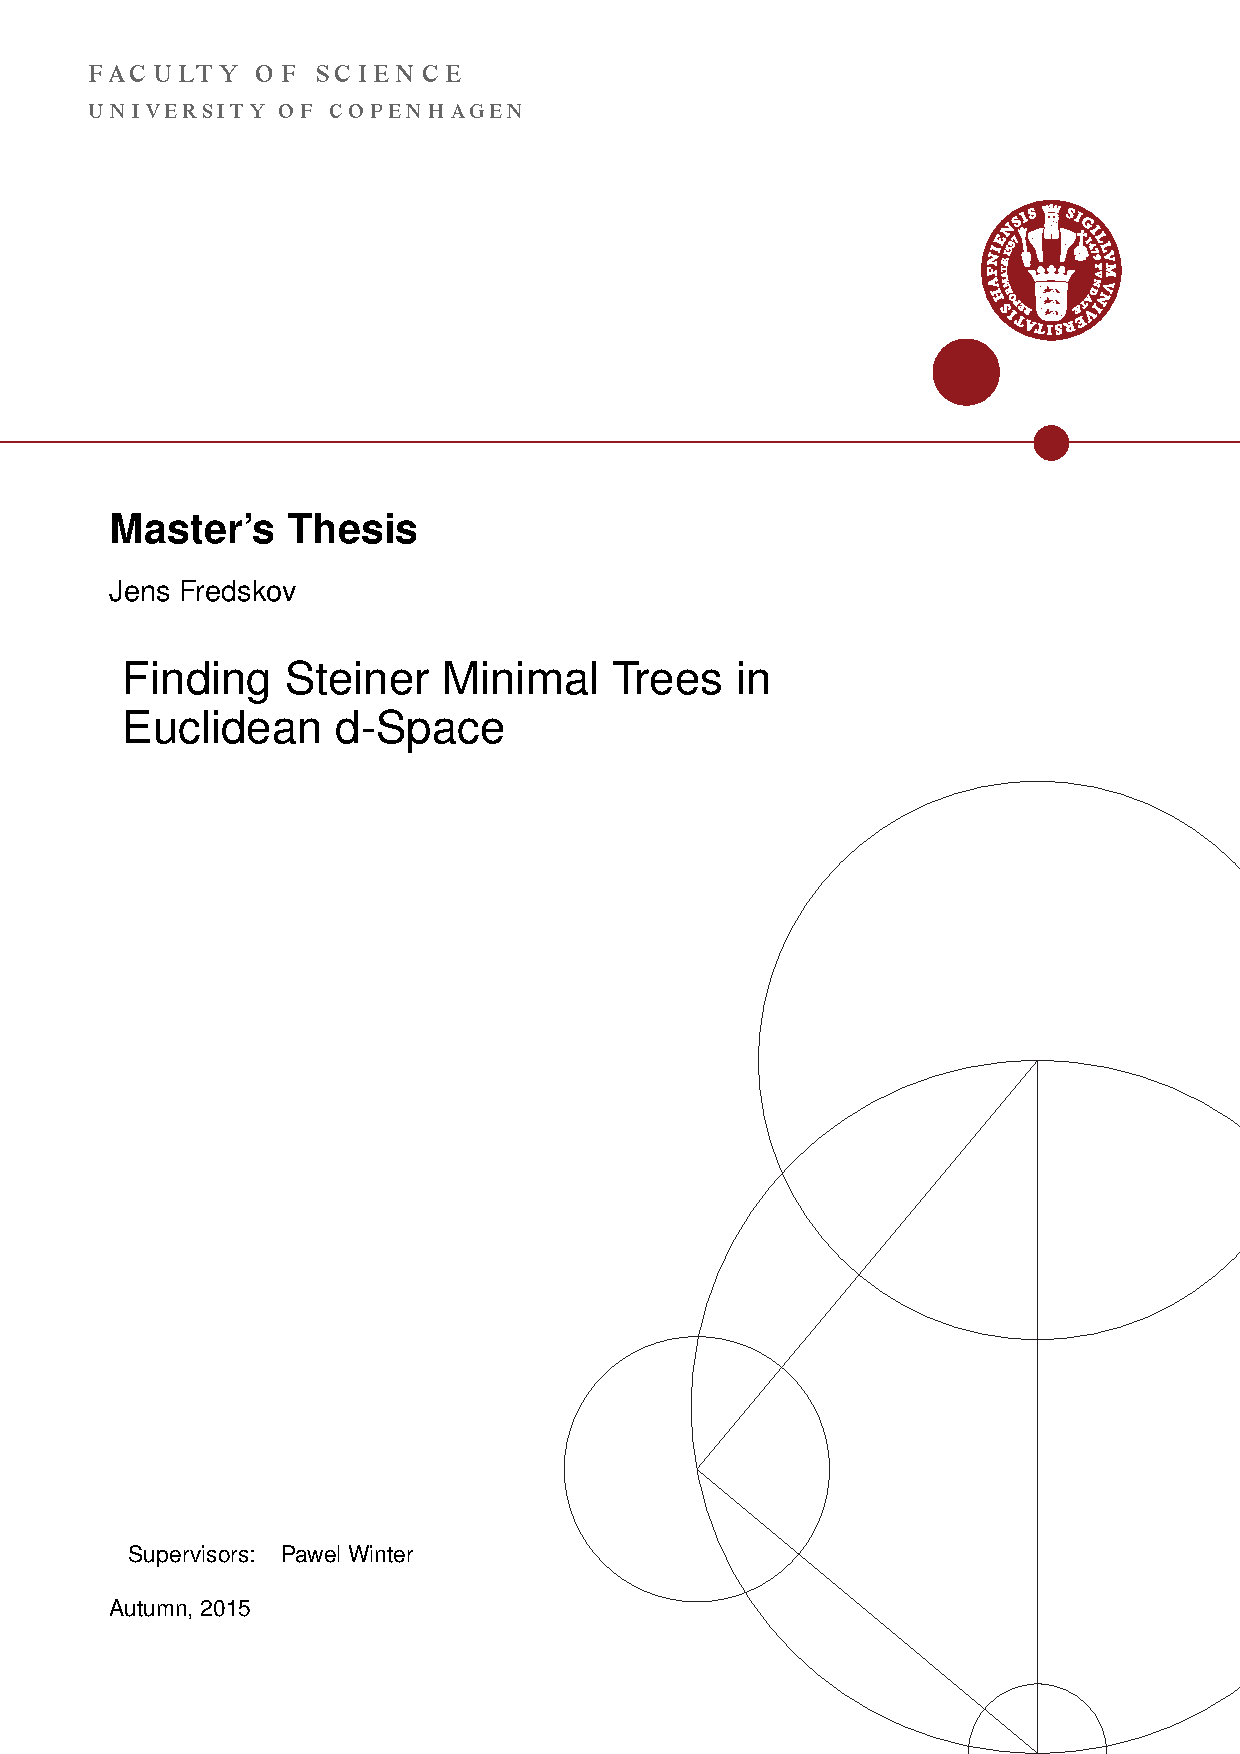
\includepdf{coverpage/coverpage}

\pagenumbering{roman} % Roman page numbering prior to the start of the thesis content (i, ii, iii, etc)

{
\abnormalparskip{0pt}
\chapter{Abstract}
\label{cha:abstract}
}

%%% Local Variables:
%%% mode: latex
%%% TeX-master: "../main"
%%% End:


{
\openany%
\listoftodos%
\newpage
\tableofcontents
\newpage
\listoftables
\newpage
\listoffigures
\newpage
\listoflistings%
\newpage
% Acronyms
\newacronym{smt}{SMT}{Steiner minimal tree}
\newacronym{rmt}{RMT}{relatively minimal tree}
\newacronym{estp}{ESTP}{euclidean Steiner tree problem}
% \newacronym{mst}{MST}{minimum spanning tree}
\newacronym{fst}{FST}{full Steiner tree}
\newacronym{fstp}{FST}{full Steiner topology}
% \newacronym{bnb}{BnB}{branch and bound}

%%% Local Variables:
%%% mode: latex
%%% TeX-master: "../main"
%%% End:

\openright%
}

%------------------------------------------------------------------------------
%	THESIS CONTENT - CHAPTERS
%------------------------------------------------------------------------------

\mainmatter%

\pagenumbering{arabic} % Arabic page numbering for thesis content (1, 2, 3, etc)

{
\abnormalparskip{0pt}
\chapter{Introduction}
\label{cha:introduction}
}

% Introduction to the thesis

\section{Objectives}
\label{sec:objectives}

% The objectives

\section{Related work}
\label{sec:related-work}

2D: geosteiner, efficient algorithms for 2d

nD: smiths, smiths+, smiths*, other?

other: interesting versions of trees, rectilinear, or multiangle version

% Any related work

\section{Structural outline}
\label{sec:structural-outline}

% the overall outline of the thesis – each chapter and its contents

\chapterbreak{}

%%% Local Variables:
%%% mode: latex
%%% TeX-master: "../../main"
%%% End:

{
\abnormalparskip{0pt}
\chapter{Preliminaries}
\label{cha:preliminaries}
}

% Short introduction to the chapter (max 1/2 page)
The following chapter introduces basic concepts and definitions which either
help in understanding the problem area of the thesis, or which are directly used
by the thesis. The most important keywords of this chapter, which are directly
used in the thesis, are:
%
\begin{itemize}
\item Topologies and trees
\item Steiner trees: \aclp{fst}, \aclp{smt}
\item \aclp{estp}
\item Fermat-Torricelli point/problem
\end{itemize}
%
At the same time this chapter will introduce versions of the Steiner tree
problem which are not used directly by the thesis, but which help to give an
understanding of the problem area of the thesis, and which are mentioned in
\cref{cha:introduction} or discussed in \cref{cha:discussion}.

This chapter is mostly based on~\textcite{smith1992,gilbert1968,brazil2015} and
will by large follow the structure of~\cite[ch.~1]{brazil2015}.

\section{The Fermat-Torricelli Problem}
\label{sec:ferm-torr-probl}

Before introducing the Steiner problem, it is relevant to introduce the
Fermat-Torricelli problem, as this can be seen as a sort of subproblem to be
solved when solving the Steiner tree problem.

\newpage

The Fermat-Torricelli problem\footnote{The problem is so named as it was first
  proposed by \textcite{fermat1891} and the earliest known solution was put
  forth by \textcite{torricelli1919}.} in its classical two dimensonal form, is
defined as follows:
%
\begin{center}
\begin{tabular}{rp{9cm}}
  \toprule
  \textbf{Given} & A set of three points $V = \{p_1, p_2, p_3\}$ lying in the plane. \\
  \textbf{Find}  & A point $s$ such that the sum of the Euclidean distances from
                   $s$ to $p_1, p_2$ and $p_3$ is minimized. \\
  \bottomrule
\end{tabular}
\end{center}
%
The point $s$ will be referred to as a Steiner point\footnote{In the
  Fermat-Torricelli problem this point would normally be named the Fermat point
  or the Fermat-Torricelli point. However for clarity as to the connection
  between this problem and the Steiner problem this term is used. The name of
  both the Steiner problem/tree/point is named after Jakob Steiner, which might
  be errornous, who supposedly studied the Steiner problem for $3$
  terminals~\cite{brazil2014}.}. There are several ways to solve this problem,
e.g.\ using the rotation-proof~\cite[p.~3--5]{brazil2015}.

This formulation of the problem can be seen as a specialized instance of the
more general problem, where the edges are weighted. In the classical version the
weight of the edges are all equal to each other.

The generalized version for two dimensions of the problem can be formulated as in
\textcite{uteshev2014}:
%
\begin{center}
  \begin{tabular}{rp{9cm}}
    \toprule
    \textbf{Given} & Three non-colinear points $p_1 = (x_1, y_1)$, $p_2 = (x_2,
                     y_2)$ and $p_3 = (x_3, y_3)$ in the plane. \\
    \textbf{Find} & The point $p_\ast = (x_\ast, y_\ast)$ which gives a solution
                    to the optimization problem
                    \begin{gather}
                      \min_{(x,y)} \sum_{j=1}^3 m_j \sqrt{{(x-x_j)}^2 + {(y-y_j)}^2}
                    \end{gather}
    Where the weight of $j$th point, $m_j$, is a real positive number. \\
    \bottomrule
  \end{tabular}
\end{center}
%
The generalized Fermat-Torricelli problem can be even further generalized from
two dimensions to $d$ dimensions, with $d \ge 2$
\cite{fermattorricelliproblem}. This simply requires the points to be
$d$-dimensional and the optimization problem to be changed to the following:
%
\begin{gather}
  \min_{(x_1, x_2, \ldots, x_d)} \sum_{j=1}^3 m_j
  \sqrt{\sum_{i=1}^d {(x_i - x_{(j,i)})}^2 }
  \\ \Updownarrow \\
  \label{eq:4}
  \min_{(p)} \sum_{j=1}^3 m_j | p p_j |, \quad p \in \mathbb{R}^d
\end{gather}
%
Solving the Fermat-Torricelli problem with even weights is equivalent with solving
the smallest possible instance of the \acl{estp}. The analytical solution
presented by~\textcite{uteshev2014} and a generalization of it to $\mathbb{R}^d$ is
presented in \cref{sec:analyt-solut-ferm}.

\section{The Euclidean Steiner Tree Problem}
\label{sec:eucl-stein-tree}

We firstly define a graph $G = (V(G), E(G))$ where the vertices $V(G)$ are
points of the graph, $V(G) \subset \mathbb{R}^d$ and the edges
$E(G) \subset (\mathbb{Z}^{+} \times \mathbb{Z}^{+})$ are straight lines
connecting the points in $V(G)$. The euclidean length of edge $e \in E(G)$ we
denote $|e|$.

The \ac{estp} is then defined as follows:
%
\begin{center}
  \begin{tabular}{rp{9cm}}
    \toprule
    \textbf{Given} & A set of points $R = \{ p_1, p_2, \ldots, p_n \}$ in
                     $\mathbb{R}^d$. \\
    \textbf{Find} & A graph $T = (V(T), E(T))$ such that $R \subseteq V(T)$, and
                    $|T| = \sum_{e \in E(T)} |e|$ is minimized. \\
    \bottomrule
  \end{tabular}
\end{center}
%
Note that $T$ must be a tree, as any cycles can obviously be removed without
disconnecting the graph or increasing the length. An example of the difference
between the \ac{mst} and \ac{smt} can be seen in \cref{fig:points-mst-smt}.
%
\begin{figure}[htbp]
  \centering
  \includegraphics[width=0.5\textwidth]{gfx/tikz/points-mst-smt}
  \caption[\acs{mst} vs. \acs{smt}]{Example of the difference between the \acs{mst} (left)
    and \acs{smt} (right) for the three points $p_1 = (0,0), p_2 = (0, 2), p_3 = (2,
    1)$. The \acs{mst} simply interconnects the existing points with the shortest
    possible tree. The \acs{smt} however adds an extra point $s_4 = (0.577, 1)$
    and interconnect these four points with the shortest possible tree. The is
    not way to interconnect the three original points with a shorter tree, no
    matter the number of extra points we add than in the left
    tree.\label{fig:points-mst-smt}}
\end{figure}

\section{Steiner Minimal Tree}
\label{sec:steiner-minimal-tree}

We define a \ac{smt} as in \textcite{brazil2015}, which is as follows:
%
\begin{definition}[\acl{smt}, Steiner points, terminals]
  A tree $T = (V(T), E(T))$ representing a solution to the Steiner tree problem
  is called a \acl{smt}. The given points $R \subseteq V(T)$ are called
  terminals and possible extra vertices $S = V(T) \setminus R$ are called
  Steiner points.
\end{definition}
%
The definition used by \textcite{smith1992} is simply that a \ac{smt} on $n$
terminals is the shortest tree containing the terminals. This definition, while being
a bit more convoluted, is essentially the same as the one given by
\textcite{brazil2015}. Thus we use that definition as it is more verbose and
gives a definition of Steiner points and terminals as well.

\section{Topologies}
\label{sec:topologies-1}

A topology is the combinatorial structure of a tree, or other form of geometric
network. This means that in a topology only the adjacencies of points
matter. Thus we could represent the topology of the tree $G = (V(G), E(G))$ as
just the edges of the tree $E(G)$ and any graph (and tree) has an
underlying topology.

We call any tree of some topology non-degenerate if all edges of the tree have
non-zero length---otherwise the tree is called degenerate.

We now define a Steiner topology and a full Steiner topology as the following:
%
\begin{definition}[Steiner topology, full Steiner topology]
The topology of a non-degenerate \ac{smt} is called a Steiner topology. The
topology of a non-degenerate \ac{smt} in which every terminal has degree 1 is
called a full Steiner topology.
\end{definition}
%
Notice that a full Steiner topology must necessarily have the most possible
Steiner points so $ k = n - 2$. This can be seen by substituting $n_2 = n_3 = 0$
and $n_1 = n$ in \cref{eq:22}.

\section{Steiner Trees}
\label{sec:steiner-trees}

Before defining Steiner trees we define \acp{rmt} as in~\cite{gilbert1968}
as:
%
\begin{definition}[\acl{rmt}]
  A tree is called a \acl{rmt} if it is the shortest possible tree of its
  underlying topology.
\end{definition}
%
As can easily be seen a \ac{smt} must also be a \ac{rmt} of its underlying
topology. Finally we define Steiner trees. Steiner trees currently have two
definitions which are not exactly identical.

The first is the definition used by \textcite{gilbert1968}, combined with the
definition for \acp{fst} in \textcite{smith1992}, is as follows:
%
\begin{definition}[Steiner tree, \acl{fst}]
  If a tree can be shortened no further even when splitting is allowed, the tree
  is called a Steiner tree. If all of the original points\footnote{I.e.\ the
    points not inserted when splitting. These are what we have so far referred
    to as the terminals.} of a Steiner tree have degree 1 the tree is called a
  \acl{fst}.\label{def:steiner-tree}
\end{definition}
%
Here the process of splitting referred to is exactly what we do when e.g.\
inserting an extra point in the Fermat-Torricelli problem. Thus it follows
pretty straightforward that a Steiner tree must also be a \ac{rmt} of the
topology which describes it\footnote{Note that here we refer to the topology we
  end up with after we cannot split any more points, and not the topology we
  started out with.}. Furthermore any \ac{smt} must also be a Steiner tree, but
not vice versa as illustrated by \cref{fig:steiner-smts}.
%
\begin{figure}[htbp]
\centering
\includegraphics[width=0.6\textwidth]{gfx/tikz/steiner-smts}
\caption[Example of splitting and \acsp{rmt}]{Example of how of splitting a point
  and inserting a new Steiner point. The flow shows two of the paths splitting
  could take on the shown topology down until no more splitting is
  possible. Optimizing the two final topologies, both are obviously \acsp{rmt} of
  their underlying topology, but only the right one is a \acs{smt} as the other
  topology is degenerate (the two Steiner points lie on top of each other in the
  center). Thus if the original points are the terminals, only the last right
  tree is a \acs{smt} for the original terminals.\label{fig:steiner-smts}}
\end{figure}
%
The other, and newer definition, used by \textcite{brazil2015} is as follows:
%
\begin{definition}[Steiner tree, \acl{fst}]
  A non-degenerate (full) \ac{rmt} for a Steiner topology is called a (full)
  Steiner tree.\label{def:steiner-tree2}
\end{definition}
%
These definitions are not exactly identical as e.g.\ the last tree to the left
in \cref{fig:steiner-smts} would not be a Steiner tree by
\cref{def:steiner-tree2}\footnote{As it has an edge of length zero.}  but would
be by \cref{def:steiner-tree}. The similarities of the two definitions should
however be obvious, and it also holds for both of the definitions that any
\ac{smt} must be a Steiner tree, and that any Steiner tree must be a \ac{rmt} of
its underlying topology. The one we will use in general is
\cref{def:steiner-tree2}.

Finally there is also the definition used by
\textcite{smith1992}, which defines a Steiner tree, by some properties which it
must also have for it to satisfy the above definitions. This is as follows
%
\begin{definition}[Steiner tree]
\leavevmode\vspace{-\baselineskip}\par
\begin{enumerate}
\item It contains $n$ terminals
  $R = \{ p_1, p_2, \ldots, p_n \} \in \mathbb{R}^d$, and possibly $k$
  additional Steiner points
  $S = \{ p_{n+1}, \ldots, p_{n+k} \} \in \mathbb{R}^d$.
\item Each Steiner point has degree $3$, the edges emanating from it are
  coplanar and have a mutual angles of $120^{\circ}$.
\item Each terminal has degree at most $3$.
\item $0 \le k \le n-2$.
\end{enumerate}
\end{definition}
%
\begin{proof}
The first property is by definition, to name the terminals and the
Steiner points.

The second and third property can be shown in the following way: First consider
that any Steiner point must have at least degree $3$. This should be obvious as
a Steiner point with degree $1$ does not connect any terminals to the rest of
the tree, and thus the point can simply be removed to either shorten the tree or
keep it the same\footnote{Which could happen if a Steiner point was lying atop
  the point is connected to.}. Furthermore every Steiner point with a degree of
$2$ can be removed, and its edges be replaced with one edge that is of the same
length or shorter as per the Triangle Inequality
Theorem\cite{triangleinequality}.

We now show that no pair of edges emanating from a Steiner point can have a
mutual angle less than $120^{\circ}$. This can be proven in a few different
ways. The one used by \textcite{gilbert1968} is based on the mechanical model
presented described in the same article. A simpler approach in my own opinion
however is the one used by \textcite{brazil2015}. The proof is follows: Consider
a point $a$ in $T$, and a pair of non-zero edges $ab, ac \in E(T)$ meeting at
$a$. Note that $ab$ and $ac$ must form a shortest interconnection of the points
$\{a, b, c\}$ and furthermore we know that a solution the Fermat-Torricelli
problem for $\{ a, b, c \}$ forms a shortest interconnection as well. An
immediate consequence\footnote{This stems from the fact that the
  Fermat-Torricelli problem has a solution at one of the points if any of the
  angles is greater than $2 \pi / 3$ and somewhere between them otherwise. The
  details can either be found in \textcite[ch.~1]{brazil2015} or somewhat
  implicitly in \cref{sec:analyt-solut-ferm}.} of this is that the angle between
$ab$ and $ac$, denoted $\angle bac$ must be at least $2 \pi / 3 = 120^{\circ}$.
To see that this is true, assume that it is smaller; We then have two cases as
shown in \cref{fig:preliminaries-steiner-point} and in neither cases is $ab$ and
$ac$ a shortest interconnection of $\{a, b, c\}$.

\begin{figure}[htbp]
\centering
\includegraphics[width=0.6\textwidth]{gfx/tikz/preliminaries-steiner-points}
\caption[Obtaining shorter trees]{Replacing a pair of edges $ab$ and $ac$ for
  which $\angle bac < 2 \pi / 3$ with a shortest interconnection provided by a
  solution to the Fermat-Torricelli problem for $\{a,b,c\}$. The left figure has
  no angle greater than $120^{\circ}$. The right has a angle $\angle cba \ge
  120^{\circ}$. In both cases a shorter tree is constructed. This figure is the
  same as in
  \textcite[p.~7]{brazil2015}.\label{fig:preliminaries-steiner-point}}
\end{figure}

Using that the mutual angles may be no less than $120^{\circ}$ it follows that
any point in $T$ can have at most degree $3$\footnote{As
  $3 \cdot 120^{\circ} = 360^{\circ}$ meaning that there is at most room for
  three edges around a point.}. It therefore follows that terminals have a
degree of at most $3$, which proves the third property, and that Steiner points
have a degree of exactly $3$ and thus also mutual angles of precisely
$120^{\circ}$, proving the second property.

The fourth property follows in the following way from property 3 and 4. Any tree
$T$ has $|V(T)|-1$ edges. Thus a Steiner tree has $n+k-1$ edges.  Every edge has
two endpoints meaning there are $2 n + 2 k - 2$ edges. As every Steiner point
has a degree of $3$, they account for $3 k$ of the endpoints. For the terminals
we must split them in three groups: $n_1$, those that have a degree of
$1$. $n_2$, those that have a degree of $2$ and, $n_3$, those that have a degree
of $3$. The terminals thus account for the rest of the endpoints, written as
$n_1 + 2 n_2 + 3 n_3 \ge n$. We can then write the equation as
%
\begin{align}
  \label{eq:22}
  3 k + n_1 + 2 n_2 + 3 n_3 &= 2 n + 2 k - 2 \\
  k &= 2 n - 2 - (n_1 + 2 n_2 + 3 n_3) \\
  0 \le k &\le n - 2
\end{align}
%
Thus proving the fourth property.
\end{proof}

\section{Finding Steiner Trees in 2D}
\label{sec:find-stein-trees-2}

In general the problem of finding \acp{smt} is NP-hard. This however is only a
measure of the worst-case upper bound. Thus in some cases it may indeed be
possible to find them much faster.

In two dimensions algorithms exists, which in many cases can find the \acp{smt} much
faster than the worst-case scenario.

This section will give a short introduction to the Hwang-Melzak and GeoSteiner
algorithm. Afterwards the section will discuss why these algorithms do not
generalize to dimensions higher than two.

\subsection{The Hwang-Melzak Algorithm}
\label{sec:hwang-melz-algor}

The Hwang-Melzak algorithm was first presented by \textcite{melzak1961} and
later improved by \textcite{hwang1986hexagonal}. For a proof of correctness see
\textcite{hwang1986linear, melzak1961}.

The algorithm is used for optimizing the tree $T$ of a pre-specified full
Steiner topology $\mathcal{T}$ with at least $n \ge 5$ terminals, assuming that
$T$ is non-degenerate. The algorithm can be implemented to run in
$\mathcal{O}(n)$. The algorithm is very well-known, and is also presented in
\textcite{brazil2015,smith1992}.

Before describing the algorithm, we define an equilateral point.
%
\begin{definition}{Equilateral point}
  An equilateral point $e_{ab}$, of the points $a$ and $b$, is a point such that the
  triangle $\triangle a b e_{ab}$ is equilateral. It is clear that in two dimensions
  such a point has two unique placements, one on each side of the line passing
  through $a$ and $b$.
\end{definition}
%
The algorithm consists of two steps. The first, the \textit{merging} step, works
as follows: Let $u$ be a Steiner point connected to $a$, $b$ and $s$, where $a$
and $b$ are terminals\footnote{It can be proven, that such a pair can always be
found. However intuitively it also makes sense, by simply thinking about the
number of terminals and Steiner points in a full Steiner topology, and realizing
that no Steiner point can be connected solely to other Steiner points, and thus
we must be able to find such a point.}. Replace $a$, $b$ and $u$ with a the
equilateral point $e_{ab}$ of $a$ and $b$. Do this $n-2$ times until the
topology consists of only $2$ points. The second step, the
\textit{reconstruction} step, works a follows: Let $\mathcal{T}'$ be the full
Steiner topology on the $n-1$ new terminals\footnote{I.e.\ the same set of
  terminals as before, but where $a$ and $b$ has been replace with
  $e_{ab}$}. Then the coordinates of $u$ can be found by taking the intersection
between the Steiner arc $\widehat{ab}$\footnote{The arc between $a$ and $b$ on the
  circle circumscribing the triangle $\triangle a b e_{ab}$.} and the edge
$e_{ab}s$. Do this on the $2$ point tree $n-2$, reinserting the points
represented by the equilateral points, until we again have a tree of $n$
terminals with the correct coordinates for the $n-2$ Steiner points.

It may well be that $\widehat{ab}$ and $e_{ab}s$ do not intersect, if this is
the case, the algorithm halts, and no solution exists for the given full
Steiner topology.

The biggest issue of the above algorithm is deciding on which side of the line
$ab$ we should place the equilateral point $e_{ab}$. However it turns out that
by choosing the order in which we perform the merging steps we are always able
to find the correct side. Thus this algorithm runs in $\mathcal{O}(n)$.

\NOTE[inline]{If time add a more detailed description of how we decide side of
  equilateral point, and add a figure of the two steps of Hwang-Melzak.}

The proof of the algorithm and how to decide the side for the equilateral point
can be found in \textcite[ch.~1]{brazil2015}.

The algorithm unfortunately does not generalize from two dimensions to higher
dimensions. The reason for this is, that while the edges emanating from a
Steiner point are indeed coplanar, the plane the points lie in is not known in
advance if there are more than $3$ terminals. This means that we no longer have
a unique pair of equilateral points for each cherry\footnote{A pair of terminals
  adjacent to a common Steiner point in a Steiner topology is called a cherry
  for the topology.}, but instead a continuous range of equilateral points lying
on a circle in $d$-space, as illustrated by \cref{fig:equi-points}.
%
\begin{figure}[htbp]
  \centering
  \begin{subfigure}[t]{0.4\textwidth}
    \includegraphics[width=\textwidth]{gfx/tikz/equi-points-2d}
    \caption{When $d = 2$ we have exactly two unique possible
      placements.\label{fig:equi-points-2d}}
  \end{subfigure}\\hspace{1em}%
  \begin{subfigure}[t]{0.4\textwidth}
    \includegraphics[width=\textwidth]{gfx/tikz/equi-points-3d}
    \caption{When $d \ge 3$ we have a circle in $d$-space of possible
      placements. Here $d = 3$ is shown.\label{fig:equi-points-3d}}
  \end{subfigure}
  \caption[Equilateral points in 2D and $d$-space]{The case where $d = 2$ only
    has the two unique possible placements of the equilateral point $e_{ab}$ for the
    two points $a$ and $b$, one of which can be eliminated when running the
    algorithm. However when $d \ge 3$ this is no longer the case, and we are
    unable to determine a unique placement of the equilateral
    point.\label{fig:equi-points}}
\end{figure}
%
Thus in contrast to the two dimensional case where we can select one of the two
unique equilateral points, in higher dimensions we are no longer able to do
this, and the algorithm breaks down.

\subsection{The GeoSteiner Algorithm}
\label{sec:geosteiner-algorithm}

\NOTE[inline]{if time add figure.}

The GeoSteiner algorithm was originally proposed by \textcite{winter1985}. Later
improvements of the implementation have allowed for the computation of \acp{smt}
for several thousand terminals~\cite{brazil2015}.

The GeoSteiner algorithm is pretty involved, and will thus not be described in
greater detail here. In general the algorithm has two phases. In the first
(\textit{generation}) phase, \acp{fst} for all full Steiner topologies of all
subsets of terminals are generated. This enumeration can be said to be done
implicitly\footnote{as opposed to explicitly defining each \ac{fst} one at a
  time.} by simulating the Hwang-Melzak algorithm, and using geometric
properties to prune parts of the Steiner arcs on which the Steiner points can
lie. In this way the algorithm can prune \acp{fst} of full Steiner which cannot
be part of the final \ac{smt}, and if all \acp{fst} of a full Steiner topology
is pruned, i.e.\ if no feasible part of a Steiner arc is left, the entire full
Steiner topology can be pruned. The strength of the algorithm lies partly in
generating \acp{fst} with similar full Steiner topologies in a single pass and
partly in being able to prune partially constructed full Steiner topologies. In
the second, (\textit{concatenation}) phase, the algorithm selects a subset of
not pruned \acp{fst} that span all terminals and has the minimum total
length. This concatenation can be formulated as the minimum spanning tree
problem in a hypergraph, which is indeed also NP-hard. However using a
branch-and-cut algorithm most instances can be solved quite
effectively\footnote{For an implementation of GeoSteiner see e.g.\
  \url{http://www.diku.dk/hjemmesider/ansatte/martinz/geosteiner/}.}. For a
fuller description of the algorithm, see e.g.\ \textcite[sec.~1.4]{brazil2015}.

While the algorithm is the most effective currently known for $d = 2$, it is
unfortunately not applicable when $d \ge 3$. First, the generation of \acp{fst}
for all subsets of terminals in $\mathbb{R}^d, d \ge 3$, is much more difficult
than in $\mathbb{R}^2$. Optimizing a \ac{fst} with more than $3$ terminals when
$d \ge 3$ requires solving high-degree polynomials~\cite{smith1992}. As a
consequence of this we can never use a algorithm such as Hwang-Melzak, but must
use numerical approaches, such as \citeauthor{smith1992}'s optimization routine
described in \cref{cha:algorithm}. Such numerical approaches seem to block the
generation of \acp{fst} across various subsets of terminals. Furthermore many of
the geometrical properties used to prune seems to be much weaker when
$d \ge 3$~\cite{fonseca2014}.

Finally \textcite[p.~142]{smith1992} describes, that it seems when $d \ge 3$,
that the topology of a \ac{smt} often consists of only a single large \ac{fst}
involving all $n-2$ Steiner points, instead of many small edge-disjoint
\acp{fst}. Whether this is true, is not really qualified by
\textcite{smith1992}, but it does seem likely that the \acp{fst} will tend to
grow larger when we get to higher dimensions, as we have more space in which
the Steiner point can lie. Thus we will not be able to leverage the benefits of
the two phases in GeoSteiner, as the \acp{fst} we generate in the first phase
will span a large portion of the set terminals, or possibly even the entire
set, making that phase very large and the second phase trivial.

\section{Finding Steiner Trees in $d$-Space}
\label{sec:find-stein-trees-d}

As described in \cref{sec:geosteiner-algorithm} determining \acp{fst} in
$\mathbb{R}^d, d \ge 3$ requires solving high-degree polynomials, and thus we
need to resort to numerical approaches.

The most well-known of these is \citeauthor{smith1992}'s algorithm, proposed by
\textcite{smith1992}. This algorithm is described in much greater detail in
\cref{cha:algorithm}, but in general it works by enumerating all full Steiner
topologies and then optimize these using an iteration which
converges to the \ac{fst} of that full Steiner topology. The algorithm can be
implemented with a branch-and-bound approach\footnote{The approach is not
  completely classic branch-and-bound as we are only able to bound, after having
  generated a complete solution. We do however generate small sub-problems of
  fewer terminals, and using the found bounds are able to prune these and their
  entire tree descendants/solutions. Thus in this way the algorithm can indeed
  be seen as branch-and-bound. The details of this can be found in
  \cref{cha:algorithm}.}, such that the found \acp{fst} can be used to prune
full Steiner topologies before optimizing them. The algorithm however cannot
solve problem instances with more than around $15$ to $20$ terminals within a
feasible amount of time.

There have been several attempts at optimizing \citeauthor{smith1992}'s
algorithm to improve its speed and thus increase the number of terminals
feasible to solve. Some of these are

\begin{itemize}
\item \textcite{fampa2008} proposed using lower bounds on partial Steiner
  topologies\footnote{I.e.\ topologies that do not include all $n$ terminals.}
  to prune \acp{fst}. Roughly the method works in the following way: Imagine we
  have a \ac{fst} not connecting all $n$ terminals. To select the next terminal
  to connect to the topology we compute the lower bounds
  $z^{\ast}(\bar{D}_l^{+})$ of every terminal not yet connected, and select the
  terminal for which the largest number of descending topologies can be
  pruned. In this way the lower bound allow \citeauthor{fampa2008} to both prune
  some descendants of topologies, and also vary the order in which they connect
  terminals to reduce the number of topologies they need to optimize. The conic
  formulation and the actual lower bound will not be discussed here as they are
  rather extensive. The method shows some improvement on both the number of
  topologies enumerated and the actual running time. However as pointed out by
  \textcite{fonseca2014} while a smaller number of \acp{fst} are generated,
  the time spent on computations increase significantly, and thus the speed
  gained from computing these lower bounds is minimal when compared to e.g.\
  distance-based sorting of the terminals.
\item \textcite{vanlaarhoven2013} proposed both a method for sorting the
  terminals by their distance to the centroid and a set of geometric criteria
  used to prune non-optimal \acp{fst}. The use of geometric criteria is partly
  what makes the 2D algorithms so successful, and thus it seems natural to
  explore these for the $d$-space case as well. However again as noted by
  \textcite{fonseca2014} these computations give very little when compared to
  simply sorting the terminals based on distance in terms of speed vs.\ time
  spent on computations.
\item \textcite{fonseca2014} proposed a way of sorting the terminals, such that
  the first three terminals maximized the sum of their pairwise distance, and
  all terminals afterwards maximize the sum of their distances to the already
  spanned terminals.
\end{itemize}

\NOTE[inline]{If time, add
  \url{http://www.iasi.cnr.it/aussois/web/uploads/2015/papers/fampam.pdf}}

Finally \textcite{fonseca2014} has also proposed a new branch enumeration
algorithm, instead of \citeauthor{smith1992}'s algorithm. This algorithm draws
its inspiration from the GeoSteiner algorithm. Instead of enumerating full Steiner
topologies and optimizing their respective trees it creates branches of subsets
of terminals. The algorithm utilizes that upon removed a Steiner point from a
full Steiner topology, $3$ branches are created, and that one can always find a
Steiner point, such that the branches have at most $\lfloor \frac{n}{2} \rfloor$
terminals, which reduces the number of branches that need to be generated. The
algorithm then consists of three phases. First, it computes \acp{smt} for subsets
with up to $8$ terminals. Second, it generates branches containing up to
$\lfloor \frac{n}{2} \rfloor$ terminals, and the \acp{smt} found in the first
phase are used to prune away branches that cannot be part of the final
\ac{smt}. Finally it generates full Steiner topologies with $n$ terminals by
concatenating three disjoint branches. The shortest tree found is then
outputted. \citeauthor{fonseca2014} noted that the branch enumeration algorithm
was able to solve many of the tested topologies with $15$ terminals within the
given time of 12 hours which \citeauthor{smith1992}'s, even with terminal
sorting, was not.

There has also been some work into heuristics and approximation algorithms. This
is however somewhat limited, and out of scope for this thesis as we here mainly
focus on \citeauthor{smith1992}'s algorithm and exact algorithms.

\section{Variations on the Steiner Tree Problem and Applications}
\label{sec:vari-stein-tree}

Steiner trees can of course be modified in several different ways. One could
think of changing both the metric, the constraints, the cost function and so
on. Some of the more well-known, are presented here with reference to where one
could read more about the type of Steiner tree if so desired. The section also
discuss some of the real world applications of Steiner trees, i.e.\ their
usefulness outside the academic world as more than a mathematical curiosity.

Some of the types of Steiner trees to mention are:
%
\begin{itemize}
\item \textbf{Rectilinear Steiner Tree} \quad A version of the Steiner tree in which
  edges must consist of vertical and horizontal line segments. It can be proven,
  that an edge always only needs to consist of at most a single horizontal, and
  a single vertical line segment, and thus we calculate the edge length using
  the rectilinear $\mathcal{L}_1$ norm. See e.g.~\textcite[ch.~3]{brazil2015}.
\item \textbf{Fixed Orientation Steiner Tree} \quad A version the of Steiner tree,
  which can be seen as a generalization of the rectilinear Steiner tree. In this
  version the metric used is a fixed orientation metric, meaning that edges are
  only allowed to have some fixed orientations, the rectilinear version can be
  seen as a fixed orientation version where we have two perpendicular
  orientations. See e.g.~\textcite[ch.~2]{brazil2015}.
\end{itemize}
%
Of possible applications, some more mentionable are:
%
\begin{itemize}
\item \textbf{Electronic circuits/VLSI Design} \quad Both rectilinear and fixed
  orientation Steiner trees have use in VLSI design and the realization of
  electronic circuits as described by
  \textcite[sec.~2.7,sec~3.6]{brazil2015}. When designing electronic circuits
  the wires between components can normally only be drawn in a rectilinear, or
  lately fixed orientation, matter. Thus Steiner trees can be used to pack the
  components closer. This also has uses for higher dimensions than $2$. As
  electronic components normally consists of several layers in which the wires
  can run between, thus crossing each other without shorting, the problem also
  has use in $3$ dimensions.
\item \textbf{Phylogenetics} \quad A method using $d$-space Euclidean Steiner trees
  has been proposed to be used in the determination of phylogenetic trees by
  \textcite{brazil2009}. Phylogenetic trees are used to determine the
  relationship between different species, these are represented as the leafs of
  the tree, and the interior nodes are then their ancestors. In this way one can
  represent the genetic difference of species, as their distance in the
  phylogenetic tree.
\end{itemize}
%
\textcite{brazil2015} cover several more possible variations on Steiner trees,
and applications of Steiner trees for the interested reader.

\NOTE[inline]{If time add obstacle-avoiding Steiner trees and possible uses for
  these in applications.}

%%% Local Variables:
%%% mode: latex
%%% TeX-master: "../../main"
%%% End:

\chapter{Smiths algorithm}
\label{ch:algorithm}

% Short introduction to the chapter (max 1/2 page)
The following chapter will describe the different parts of the algorithm used by
Smith~\cite{Smith1992}. \TODO{Finish introduction}

\section{Overview}
\label{sec:overview}

The algorithm in general follow the form of as proposed by Gilbert and
Pollak~\missingref{18 in Smith}

\TODO[inline]{Finish the overview}

\TODO[inline]{Add a note that while there may not have been other ways to go at
  the time, today we also have things such as the one described in Fonseca,
  Pawel, et al.}

\section{Topologies}
\label{sec:topologies}

The first step of the algorithm is, as described in \Cref{sec:overview}, to
generate topologies. It is therefore natural that we need some way of
representing and generating these topologies.

The algorithm only considers full Steiner topologies where $K = N - 2$. This is
a \NOTE{is there a better word than legal?} legal approach as we can simply
regard any Steiner tree with $K \le N - 2$ as a \ac{FST} where some edges have
length zero and thus some points have ``merged''.

\subsection{Representation}
\label{sec:representation}

\begin{figure}[htbp]
\centering
  \begin{subfigure}[b]{0.3\textwidth}
    \includegraphics[width=\textwidth]{gfx/tikz/algorithm-topology-1}
    \caption{Here be dragons.\label{fig:algorithm-topology-1}}
  \end{subfigure}
~
  \begin{subfigure}[b]{0.3\textwidth}
    \includegraphics[width=\textwidth]{gfx/tikz/algorithm-topology-2}
    \caption{Here be dragons.\label{fig:algorithm-topology-2}}
  \end{subfigure}
~
  \begin{subfigure}[b]{0.3\textwidth}
    \includegraphics[width=\textwidth]{gfx/tikz/algorithm-topology-3}
    \caption{Here be dragons.\label{fig:algorithm-topology-3}}
  \end{subfigure}
\caption[How to construct Steiner topologies]{Here be dragons.\label{fig:algorithm-topologies}}
\end{figure}

There is an 1--1 correspondence between full Steiner topologies with $N \ge 3$
regular points, and $(N-3)$-vectors $\vec{a}$, whose $i$th entry $a_i$ is an
integer between $1 \le a_i \le 2 i + 1$.

\TODO[inline]{Describe/Outline proof and the generation as shown in the figures.}

\subsection{Generation}
\label{sec:generation}

Using the representation described in \Cref{sec:representation} the problem of
generating all topologies can now be done as a backtracking problem generating
all $(N-3)$-topology vectors.

\TODO[inline]{Describe the backtracking here}

To further speed up the generation of topologies, or rather to avoid generating
unnecessary topologies, Smith also utilizes the following theorem

\begin{theorem}
For any set of $N$ distinct regular points in any Euclidean space, the length of
the shortest tree, interconnecting $N-1$ points, with topology vector $a_1
\cdots a_{N-4}$ is no greater than the length of the shortest tree,
interconnecting $N$ points, with topology vector $a_1 \cdots a_{N-3}$.
\end{theorem}

\TODO[inline]{Proof of above theorem}

The algorithm utilizes this to prune in the following way. Imagine we have found
some upper bound for the \ac{SMT}. If we then optimize any generated topology
vector which does not yet include all the regular points, and it turns out to
have length greater than the upper bound, we can prune any topologies that we
would have generated from this vector, as the length of the larger topologies
cannot become any smaller than the length of the current, and thus cannot become
smaller than the length of the upper bound.

Thus the implementation of the algorithm generates and optimizes topologies
depth-first to ensure we get a upper bound as quickly as possible. If it did
breadth-first we would not be able to prune anything, as we would get all the
full topologies as the last to optimize.

\section{Optimization of a topology}
\label{sec:optim-topol}

\TODO[inline]{TODO}

\subsection{Iteration}
\label{sec:iter-fixm-could}

\FIXME[inline]{This section could probably be better named}
\TODO[inline]{TODO}

%%% Local Variables:
%%% mode: latex
%%% TeX-master: "../../main"
%%% End:

 {
\abnormalparskip{0pt}
\chapter{Data Structures and Methods}
\label{cha:data-structures}
}

This chapter will describe some more notable elements of the new implementation,
with regard to data structures and methods not used by
\textcite{smith1992}. Specifically it describes the new data structure
introduced for holding and building topologies. It also describes the new
iteration based of the simple iteration described in \cref{sec:simple-iteration}
and using the analytical method for solving the Fermat-Torricelli problem
presented by \textcite{uteshev2014}. This also includes a description of said
method, and a generalization to $d$-space, as the one presented by
\textcite{uteshev2014} only is for 2D. Finally the chapter also describes a new
way of sorting the terminals.

\section{Building Topologies}
\label{sec:building-topologies}

In \citeauthor{smith1992}'s implementation of the algorithm when generating
topologies every new topology is rebuilt completely from the bottom. E.g.\ say
that we have just optimized the topology corresponding to the topology vector
$A = [1, 2]$. If we now wish to optimize the topology vector
$A' = [1, 2, 3]$. In the old implementation $A'$ would have to be built again
from scratch instead of simply splitting and building on to $A$.

To avoid this extra work, the new implementation instead uses a different
approach. The underlying data of a tree is in most aspects more or less
identical to \citeauthor{smith1992}'s as it is a series of arrays to hold points
and edges. However these are coupled together in a struct (in Go, the
programming language of choice, this is essentially a record on which one can add
methods.). Instead of rebuilding this entire struct every time we split or
restore the topology, it has methods to do exactly this. Thus, using the earlier
example, from $A$ we could either split an
edge and get $A'$, or any other length three topology vector having $A$ as a
prefix, or we could restore and go back from $A$ to $A'' = [1]$\footnote{From
  $A''$ we could then either split again to e.g.\ the next topology vector of
  length two, $[1, 3]$, or restore once again.}

The way this is implemented is a follows: All edges of the tree are kept in an
list, and edge being represented as the tuple $(a, b)$ meaning it starts at
point $p_a$ and ends at point $p_b$. Say we have $n$ terminals in all, and have
currently connected the $i$ first terminals. This means we have $i-2$ Steiner points
continuously enumerated from $n+1$ up to $n+i-1$ and $2i-3$ edges enumerated
continuously from $1$.

Now we wish to split some edge $e_j = (c, d)$ where $1 \le j \le 2i-3$, so any
of the existing edges, and connect the next terminal $p_{i+1}$ to the existing
topology. We do this by first changing the original edge to go from the first
end point $p_c$ to a new Steiner point $p_{n+i}$. Afterwards we append two new
edges to the list of edges, $e_{2i-2} = (d, n+i)$ and $e_{2i-1} = (i+1, n+i)$
thus connecting $p_d$ and $p_{i+1}$ to Steiner point $p_{n+i}$ as well. This
process is straight forward and if the accessing into the list and
appending\footnote{which is both the case if enough space is allocated for the
  list ahead of the appending.} is $\mathcal{O}(1)$ then the entire operation
will be $\mathcal{O}(1)$. The operation can be seen in
\cref{fig:splitting-topology}. In this way we can expand the topology one
terminal at a time without rebuilding every time.

\begin{figure}[htbp]
  \centering
  \begin{tabular}{|c|ccc|c|ccc|c|}
  \multicolumn{1}{c}{$1$}
  & \multicolumn{3}{c}{ }
  & \multicolumn{1}{c}{$i$}
  & \multicolumn{3}{c}{ }
  & \multicolumn{1}{c}{$2k + 1$}
  \\ \hhline{--~---~--}
  $(a,b)$
  & & \ldots
  & & \cellcolor{SkyBlue} \tikzmark{a} $(c,d)$
  & & \ldots
  & & $(e,f)$
  \\ \hhline{--~---~--}
\end{tabular}

\vspace{8ex}

\begin{tabular}{|c|ccc|c|ccc|c|c|c|}
  \multicolumn{1}{c}{$1$}
  & \multicolumn{3}{c}{ }
  & \multicolumn{1}{c}{$i$}
  & \multicolumn{3}{c}{ }
  & \multicolumn{1}{c}{$2k+1$}
  & \multicolumn{1}{c}{$2k+2$}
  & \multicolumn{1}{c}{$2k+3$}
  \\ \hhline{--~---~----}
  $(a,b)$
  & & \ldots
  & & \cellcolor{SkyBlue} \tikzmark{b} $(c,k+1)$
  & & \ldots
  & & $(e,f)$
  & \cellcolor{SkyBlue} \tikzmark{c} $(d,k+1)$
    & \cellcolor{SkyBlue} \tikzmark{d} $(g,k+1)$
  \\ \hhline{--~---~----}
\end{tabular}

\begin{tikzpicture}[overlay, remember picture, yshift=-1.5ex, xshift=2em]
  \draw [-{Latex[length=2mm,width=2mm]},semithick] ({pic cs:a}) [bend right] to ([yshift=6.5ex]{pic cs:b});
  \draw [-{Latex[length=2mm,width=2mm]},semithick] ({pic cs:a}) [out=-70, in=110] to ([yshift=6.5ex]{pic cs:c});
  \draw [-{Latex[length=2mm,width=2mm]},semithick] ({pic cs:a}) [out=-20, in= 120] to ([yshift=6.5ex]{pic cs:d});
\end{tikzpicture}

%%% Local Variables:
%%% mode: latex
%%% TeX-master: "../main"
%%% End:

  \caption[Implementation of topology splitting]{Splitting on edge $e_j$ with
    $i$ terminals currently connected, results in two new edges $e_{2i-2}$ and
    $e_{2i-1}$ and a change of the existing edge $e_j$. Finally we also get the new
    Steiner point $n+i$.\label{fig:splitting-topology}}
\end{figure}

The reason for this way of expanding the topology however lies with the wish to
also restore an edge. If we keep a list of all the edges we split
on\footnote{which we do, as this is the topology vector described in
  \cref{sec:representation}.} we can always restore the last edge split in the
following way. Select the last two edges, $(d, n+i), (i+1, n+i)$ in the list and
the edge $e_j = (c, n+i)$. Now change edge $e_j$ to $(c, d)$ and remove the last
two edges in the list. Thus we have $\mathcal{O}(1)$ methods for splitting and
restoring the topology, in a way which is consistent in the numbering with the
one described in \cref{sec:representation} and shown in
\cref{fig:algorithm-topologies}.

\section{Analytical Solution to the Fermat-Torricelli Problem}
\label{sec:analyt-solut-ferm}

An analytical solution for finding the Fermat-Torricelli point of three
prespecified points in 2D is presented by \textcite{uteshev2014}---which is the same as
finding the Steiner point of those three points. The article presents a
solution for two dimensions which will be described. However as we are working
in $\mathbb{R}^d$ a generalization of the solution to $d$-space is necessary and
will also be presented. This generalization is as far as I know, not presented
anywhere else in the literature.

The reason this why is interesting is that \textcite{smith1992} mentions that an
iterative process which updates points one at a time would not be as quick to
converge as the one he presents. There is however no experiments in the paper to
support this. Thus this analytical method is interesting, as it is actually not
computationally heavy to compute the location of a Steiner point, and as each
optimization moves a Steiner point to the exact location at which it minimizes
the length to its three neighbors at the time. One could therefore think that this might
actually converge quite fast.

Using this analytical solution an optimization iteration similar to the one
described in \cref{sec:simple-iteration} has been implemented. The method does
not completely follow the one described, but switches out the iteration by
\citeauthor{smith1992} with an iteration that runs over all Steiner points and
places them using the analytical method. This is due to the fact that I wished
to reuse the main loop which iterates through topologies, and that the simple
iteration in the way it is described in \cref{sec:simple-iteration} was first
finalized after the implementation of the analytical solution. Thus this method
may indeed be doing some double work of its own\footnote{E.g.\ when splitting
  the topology, the new Steiner point gets initial placement at its neighbors
  centroid slightly pertubed. This could perhaps have been improved to using the
  analytical solution as well.}, some of which will be discussed in
\cref{cha:discussion}.

\subsection{2D}
\label{sec:2d}

The solution for two dimensions is presented by \textcite{uteshev2014} is for
the generalized Fermat-Torricelli problem, which given three non-colinear points
$p_1 = (x_1, y_1)$, $p_2 = (x_2, y_2)$ and $p_3 = (x_3, y_3)$ in the plane,
finds the point $p_\ast = (x_\ast, y_\ast)$ which gives a solution to the
optimization problem
%
\begin{equation}
  \min_{(x,y)} F(x,y) \quad \text{for} \quad F(x,y) = \sum_{j=1}^3 m_j
  \sqrt{{(x-x_j)}^2 + {(y-y_j)}^2}
\end{equation}
%
Where the weight of the $j$th point, $m_j$, is a real positive number. The
instance where $m_1 = m_2 = m_3 = 1$ is exactly the classical Fermat-Torricelli
problem, which has a unique solution either coinciding with one of the points
$p_1$, $p_2$, $p_3$ or with the Fermat-Torricelli or Steiner point of the
triangle $p_1 p_2 p_3$. The instance with unequal weights is known as the
generalized Fermat-Torricelli point.

As we only need the classical version of the problem, I have decided to rewrite
the proof done by \textcite{uteshev2014} for the 2D case with the weights set to
$1$. In a lot of ways, the proof is the same, however it does become a bit
simpler and cleaner. The original proof for the generalized version can be found
in \textcite{uteshev2014}. Thus what we wish to minimize is instead the
following problem:
%
\begin{equation}
  \min_{(x,y)} F(x,y) \quad \text{for} \quad F(x,y) = \sum_{j=1}^3
  \sqrt{{(x-x_j)}^2 + {(y-y_j)}^2}
\end{equation}
%
Existence and uniqueness of the solution is guaranteed by
\cref{thm:fermat-torricelli}
%
\begin{theorem}
\label{thm:fermat-torricelli}
  Denote the corner angles of the triangle $\triangle p_1 p_2 p_3$ by $\alpha_1, \alpha_2,
  \alpha_3$. Then if the conditions
  %
  \begin{equation}
    \label{eq:12}
    \left\{
      \begin{array}{c}
        1 < 2 + 2 \cos \alpha_1 , \\
        1 < 2 + 2 \cos \alpha_2 , \\
        1 < 2 + 2 \cos \alpha_3 , \\
      \end{array}
    \right.
  \end{equation}
  %
  are fulfilled, corresponding to all angles being less than $120^{\circ}$, then
  there exists a unique solution $p_\ast = (x_\ast, y_\ast) \in \mathbb{R}^2$
  for the classic Fermat-Torricelli problem lying inside the triangle
  $\triangle p_1 p_2 p_3$. This point is a stationary point for the function
  $F(x,y)$, i.e.\ a real solution of the system
  %
  \begin{equation}
    \label{eq:13}
    \left\{
      \begin{array}{c}
        \frac{d(F(x,y))}{dx} = \sum_{j=1}^3 \frac{(x-x_j)}{\sqrt{{(x-x_j)}^2 +
        {(y - y_j)}^2}} = 0, \\
        \frac{d(F(x,y))}{dy} = \sum_{j=1}^3 \frac{(y-y_j)}{\sqrt{{(x-x_j)}^2 +
        {(y - y_j)}^2}} = 0
      \end{array}
    \right.
  \end{equation}
  %
  If any of the conditions in \cref{eq:12} is violated then $F(x,y)$ attains its
  minimum value at the corresponding vertex of triangle.
\end{theorem}
%
Calculating the coordinates of the point $(x_\ast, y_\ast)$, if the conditions
in \cref{eq:12} are fulfilled, is done as follows
\begin{gather}
  \label{eq:15}
  x_\ast = \frac{K_1 K_2 K_3}{2 \sqrt{3} S d} \left( \frac{x_1}{K_1} +
  \frac{x_2}{K_2} + \frac{x_3}{K_3} \right), \quad
  y_\ast = \frac{K_1 K_2 K_3}{2 \sqrt{3} S d} \left( \frac{y_1}{K_1} +
  \frac{y_2}{K_2} + \frac{y_3}{K_3} \right)
  \intertext{with}
  \label{eq:11}
  F(x_\ast, y_\ast) = \min_{(x,y)} F(x,y) = \sqrt{d}
  \intertext{Here}
  \label{eq:1}
  r_{jl} = \sqrt{{(x_j - x_l)}^2 + {(y_j - y_l)}^2} = |p_j p_l|
  \quad \{j,l\} \in \{ 1, 2, 3 \} \\
  \label{eq:20}
  S = | x_1 y_2 + x_2 y_3 + x_3 y_1 - x_1 y_3 -x_3 y_2 - x_2 y_1 | \\
  \label{eq:3}
  \left\{
    \begin{array}{c}
      K_1 = \frac{\sqrt{3}}{2} (r_{12}^2 + r_{13}^2 - r_{23}^2) + S
      \\
      K_2 = \frac{\sqrt{3}}{2} (r_{12}^2 + r_{23}^2 - r_{13}^2) + S
      \\
      K_3 = \frac{\sqrt{3}}{2} (r_{23}^2 + r_{13}^2 - r_{12}^2) + S
    \end{array}
  \right. \\
  d = \frac{1}{\sqrt{3}} (K_1 + K_2 + K_3) \\
\end{gather}

The proof of \cref{eq:15,eq:11} can be found in a generalized version in
\textcite{uteshev2014}, or in \cref{sec:2d-1} where it has been
adapted to the unweighted version of the problem.

\subsection{Generalization to $d$-Space}
\label{sec:gener-high-dimens}

Generalizing the solution described above to higher dimensions is in general
pretty straightforward. The biggest change is in the representation of $S$, and
the fact that the proof requires a bit of sum manipulation. This generalized
version of the proof is not known to have been presented in any paper before.

The generalization is as for the 2D variant here done for the classic
Fermat-Torricelli problem. It could however just as easily be done for the
weighted problem, by following the form of the proof in \textcite{uteshev2014}
instead of the form in \cref{sec:2d}.

The first change is that we no longer try to minimize a function of just two
parameters, but instead we intend to minimize a function of $d$ parameters,
where our points are contained in $\mathbb{R}^d$, i.e.\ we have $d$ dimensions. As we
normally represent this using vectors, we would not actually have $d$
parameters, but instead one parameter being a $d$-vector. Thus we wish to find a
point $p_\ast = (x_{(\ast,1)}, x_{(\ast,2)}, \ldots, x_{(\ast,d)}) \in \mathbb{R}^d$
which minimizes the following function for the three points
$p_1 = (x_{(1,1)}, x_{(1,2)}, \ldots, x_{(1,d)}), p_2 = (x_{(2,1)}, x_{(2,2)},
\ldots, x_{(2,d)}), p_3 = (x_{(3,1)}, x_{(3,2)}, \ldots, x_{(3,d)}) \in \mathbb{R}^d$.
%
\begin{gather}
  \min_{(x_1, x_2, \ldots, x_d)} F(x_1, x_2, \ldots, x_d) \quad \text{for} \quad
  F(x_1, x_2, \ldots, x_d) = \sum_{j=1}^3 \sqrt{\sum_{i=1}^d {(x_i -
    x_{(j,i)})}^2 }
  \\ \Updownarrow \\
  \label{eq:4}
  \min_{(p)} F(p) \quad \text{for} \quad
  F(p) = \sum_{j=1}^3 | p p_j |, \quad p \in \mathbb{R}^d
\end{gather}
%
The point $p_\ast$ now no longer has to be a solution to the equation system in
\cref{eq:13}, but to a similar system containing $d$ equations, as follows
%
\begin{equation}
\label{eq:7}
  \left.
    \begin{array}{c}
    \sum_{j=1}^3 \frac{(x_1-x_{(j,1)})}{| p p_j|} = 0
    \\
    \sum_{j=1}^3 \frac{(x_2-x_{(j,2)})}{| p p_j|} = 0
    \\
    \vdots
    \\
    \sum_{j=1}^3 \frac{(x_d-x_{(j,d)})}{| p p_j|} = 0
  \end{array}
  \right\} =
  \sum_{j=1}^3 \frac{(p - p_j)}{| p p_j |} = \vec{0}
\end{equation}
%
Then as before, if the conditions in \cref{eq:12} are fulfilled\footnote{If not
  the point is as before located at the corresponding vertex.} the solution to
\cref{eq:7} can be found as follows
%
\begin{gather}
  p_\ast = (x_{(\ast,1)}, x_{(\ast,2)}, \ldots, x_{(\ast,d)})\label{eq:8}
  \intertext{with}
  x_{(\ast, j)} = \frac{K_1 K_2 K_3}{2 \sqrt{3} S d} \left( \frac{x_{(1,j)}}{K_1} +
  \frac{x_{(2,j)}}{K_2} + \frac{x_{(3,j)}}{K_3} \right), \quad 0 < j \le d\label{eq:5}
  \intertext{and}
  F(p_\ast) = \min_{(p)} F(p) = \sqrt{d}\label{eq:21}
  \intertext{Here}
  \label{eq:14} r_{jl} = \sqrt{\sum_{i = 1}^d {(x_{(j,i)} - x_{(l,i)})}^2} = |p_j p_l|
  \quad \{j,l\} \in \{ 1, 2, 3 \} \\
  S = \frac{1}{2} \sqrt{(r_{12} + r_{23} + r_{13}) (r_{23} + r_{13}) (r_{12} +
    r_{13}) (r_{12} + r_{23})} \\
\end{gather}
%
And the rest of the expressions are the same as in the 2D version. As can be seen,
all of the expressions, except for $S$ (and the distance which now of course
have more than two dimensions), retain the same representation as in the two
dimensional version. $S$ however looks quite different. Exactly how the new $S$
is related to the old $S$ is still unclear to me. \textcite{uteshev2014}
describes, that $S$ in 2D rewritten, can be recognized as the doubled area of
the triangle $\triangle p_1 p_2 p_3$. This geometrical understanding however
seems to be missing from the higher dimension case. Indeed the idea for the
representation of $S$ stems from talks with my supervisor Pawel Winter, who
pointed me to an earlier implementation of the general case, that he has done
himself. Thus an intuition of the new $S$ is missing, however as can be seen
from the proof \cref{sec:d-space}, it does indeed work.

\section{Sorting the Terminals}
\label{sec:sorting-terminals}

The idea of sorting the terminals before one starts to build and optimize
topologies is not new, and has also been suggested by \textcite{smith1992}. The
idea behind sorting the terminals, is to find some way of sorting the terminals,
such that the initial \acp{rmt} have become as large as possible, as fast as
possible. Doing this allows us to early on see if we need to discard a topology
vector as prefix, if its \ac{rmt} is longer than the upper bound, and thus be
able to prune more topologies, than if we added terminals in an arbitrary order.

At least two different kinds of sorting has been implemented by
\textcite{fonseca2014,vanlaarhoven2013}. Both methods have shown promising
results regarding the number of trees one needs to optimize in contrast to not
sorting the terminals.

The first method, presented by \textcite{vanlaarhoven2013}, sorts the terminals
by their decreasing distance to the centroid of the set of terminals, i.e.\ the
first terminal is the farthest away, and the last terminal is the closest. A
potential issue with this way of sorting, is that while the terminals may be far
from the centroid, they can potentially still be rather close to each other,
thus not pruning much faster.

The second method, presented by \textcite{fonseca2014}, sorts the terminals such
that the first three terminals $p_1, p_2, p_3$ maximize the sum of their
pairwise distances, and $p_i, i = 4, 5, \ldots, n$ is the farthest away from
$p_1, p_2, \ldots, p_{i-1}$. This method seems to have a lot of potential as it
tries to ensure that every terminal added is as far away from the current
\ac{rmt} as possible. However one could easily think of positions for the
terminals, such that the terminals $p_4, p_5, \ldots, p_n$ all lie close to each
other, and within the first three terminals. This could mean that the distance
added every step after the initial \ac{rmt} will be spread out on the next few
steps, instead of adding as much as possible as quickly as possible.

Here another method is proposed which is relatively similar to the one proposed
and implemented by \textcite{fonseca2014}, but a lot simpler and requiring fewer
steps. The initial idea for the method was to find the longest path in a fully
connected graph, where the nodes in the graph are the terminals. This problem is
however NP-hard~\cite{longestpathproblem}, and it seems a bit silly to solve a
NP-hard problem to try and improve on a NP-hard problem. Thus the method
proposed here sorts the terminals as follows: Select the initial terminal $p_1$
arbitrarily. From there select the next terminal $p_i, i = 2, 3, \ldots, n$ such
that the distance to $p_{i-1}$ is maximized.

The idea behind this approach, is that the method is extremely easy to implement
and hopefully gives better runtimes, comparable to those of e.g.\
\textcite{fonseca2014}.

%%% Local Variables:
%%% mode: latex
%%% TeX-master: "../../main"
%%% End:

 {
\abnormalparskip{0pt}
\chapter{Implementation}
\label{cha:implementation}
}

The new implementation has been written in the, still relatively new but at this
point stable, language Go, which quoting the homepage: ``Go is an open source
programming language that makes it easy to build simple, reliable, and efficient
software.''~\cite{golanghomepage}. Go is a general-purpose, strongly typed and
garbage-collected language. The syntax bears resemblance to C\footnote{But
  with a lot less braces, and no pointer arithmetic.}. Furthermore Go has
explicit support for concurrent programming. The language furthermore sports
extremely fast compiling of source code and tries to have performance
comparable to C.

The reasoning behind choosing Go for the new implementation were firstly that I
already had experience with the language making it easy to get to work on the
new implementation without also having to learn a new programming
language. Secondly the language has, in my opinion, a very clean syntax which
makes it easily readable for anyone familiar with any C-syntax styled
language. Finally the easy use of concurrency in Go\footnote{Starting a new
  goroutine, which is the languages type of lightweight threads, is as simple as
  writing: \texttt{go~SomeFunction~(args\ldots)}.} made it interesting as
continued work with the new implementation could include a potential,
significant, speedup by making the branching of the algorithm concurrent. The
same could be be true for the Gauss elimination, concurrent\footnote{Not
  concurrency has actually been implemented in the new implementation. However
  the possibilities of this is discussed in \cref{sec:concurrency}.}.

In general the implementation tries to follow guidelines given in
\textcite{effectivego}. These are guidelines as to how one codes effective
Go. Here effective means both in terms of speed, memory usage, stability and
readability.

Source code for the new implementation, fixes for the old implementation and
experiments can be found at \url{https://github.com/jsfr/SteinerExact}. The
source code for just the new implementation is also included in
\cref{cha:source-code}.

This chapter will describe the architecture of the new implementation, i.e.\ how
the new implementation has been structured.

\TODO[inline]{Describe the source code architecture, and rewrite introduction so
it makes sense with new structure.}

\section{Main and Config File}
\label{sec:main-file}

\section{\acs{smt} Package}
\label{sec:smt-package}

\subsection{Data Structures}
\label{sec:data-structures}

\subsection{Methods}
\label{sec:methods}

%%% Local Variables:
%%% mode: latex
%%% TeX-master: "../../main"
%%% End:

{
\abnormalparskip{0pt}
\chapter{Experiments}
\label{cha:experiments}
}

Introduction, max 1/2--1 page

golang 1.4.1/2

Naming of methods:
\begin{table}[htbp]
  \centering
  \begin{tabular}{cp{9cm}}
    \toprule
    Method       & Description                                      \\
    \midrule
    Simple       & New implementation with the analytical method.   \\
    SimpleSort   & New implementation with the analytical method and sorted
                   terminals.                                       \\
    SmithNew     & New implementation with \citeauthor{smith1992}'s
                   iteration.                                       \\
    SmithNewSort & New implementation with \citeauthor{smith1992}'s iteration
                   and sorted terminals.                            \\
    SmithOld     & Original implementation by \textcite{smith1992}. \\
    \bottomrule
  \end{tabular}
  \caption[Here be dragons]{Here be dragons.\label{tab:method-names}}
\end{table}

\section{Correctness}
\label{sec:correctness}

$150$ random cubes with $n = 10 \ldots 12$ and $d = 2$.

Simple seems faulty in a few instances:

\begin{table}[htbp]
  \centering
  \begin{tabular}{ccc}
    \toprule
    Instance           & Method     & Diff        \\
    \midrule
    cube\_n12\_d2\_s27 & Simple     & $0.0032114$ \\
    cube\_n12\_d2\_s49 & Simple     & $0.0062502$ \\
    cube\_n10\_d2\_s42 & SimpleSort & $0.0002782$ \\
    cube\_n12\_d2\_s26 & SimpleSort & $0.0040131$ \\
    cube\_n12\_d2\_s43 & SimpleSort & $0.0065104$ \\
    cube\_n12\_d2\_s49 & SimpleSort & $0.0062502$ \\
    \bottomrule
  \end{tabular}
  \caption[Here be dragons]{Here be dragons.\label{tab:correctness-errors}}
\end{table}

This seems to be because the current error function is incompatible with this
iteration, as the error gets very low quickly, but may have some of the
described problems. Thus the line \texttt{q-r < upperBound} will skip some trees
which can actually become better. The same goes for the lines deciding when we
stop optimization.

\section{Speed}
\label{sec:speed}

\begin{table}[htbp]
  \centering
  \begin{tabular}{ccccc}
    \toprule
    Set     & Dimensions       & Terminals             & Set size & Point configuration \\
    \midrule
    Carioca & $d = 3 \ldots 5$ & $n = 11 \ldots 16$    & $90$       & Random in cube      \\
    Cube    & $d = 2 \ldots 4$ & $n = 10 \ldots 15$    & $360$      & Random in cube      \\
    Iowa05  & $d = 3 \ldots 5$ & $n = 10$              & $30$       & Random in cube      \\
    Sausage & $d = 2 \ldots 5$ & $n = 10 \ldots 15$    & $24$       & Simplex sequence    \\
    Solids  & $d = 3$          & $n = 4, 6, 8, 12, 20$ & $5$        & Platonic solids     \\
    \bottomrule
  \end{tabular}
  \caption[Here be dragons]{Here be dragons.\label{tab:test-sets}}
\end{table}

\begin{table}[htbp]
  \centering
  \begin{tabular}{cccccc}
    \toprule
            & \multicolumn{5}{c}{Method}                               \\
    \cmidrule(l){2-6}
    Set     & Simple & SimpleSort & SmithNew & SmithNewSort & SmithOld \\
    \cmidrule(r){1-1}\cmidrule(l){2-6}
    Carioca & $81$   & $89$       & $73$     & $87$         & $76$     \\
    Cube    & $360$  & $360$      & $352$    & $360$        & $356$    \\
    Iowa05  & $30$   & $30$       & $30$     & $30$         & $30$     \\
    Sausage & $22$   & $23$       & $18$     & $22$         & $21$     \\
    Solids  & $4$    & $4$        & $4$      & $4$          & $4$      \\
    \bottomrule
  \end{tabular}
  \caption[Here be dragons]{Here be dragons.\label{tab:set-success}}
\end{table}

All sets have been taken from \textcite{fonseca2014}, but the sets Carioca and
Cube has been pruned.

8 $\times$ Intel\textsuperscript{\textregistered}
Xeon\textsuperscript{\textregistered} CPU E5-2630L @ 2.00 GHz and 16 GB RAM

Describe why I have pruned Carioca and Cube.

Plot all five against each other on interesting sets

\begin{figure}[htbp]
  \centering
  \begin{subfigure}[t]{0.5\textwidth}
    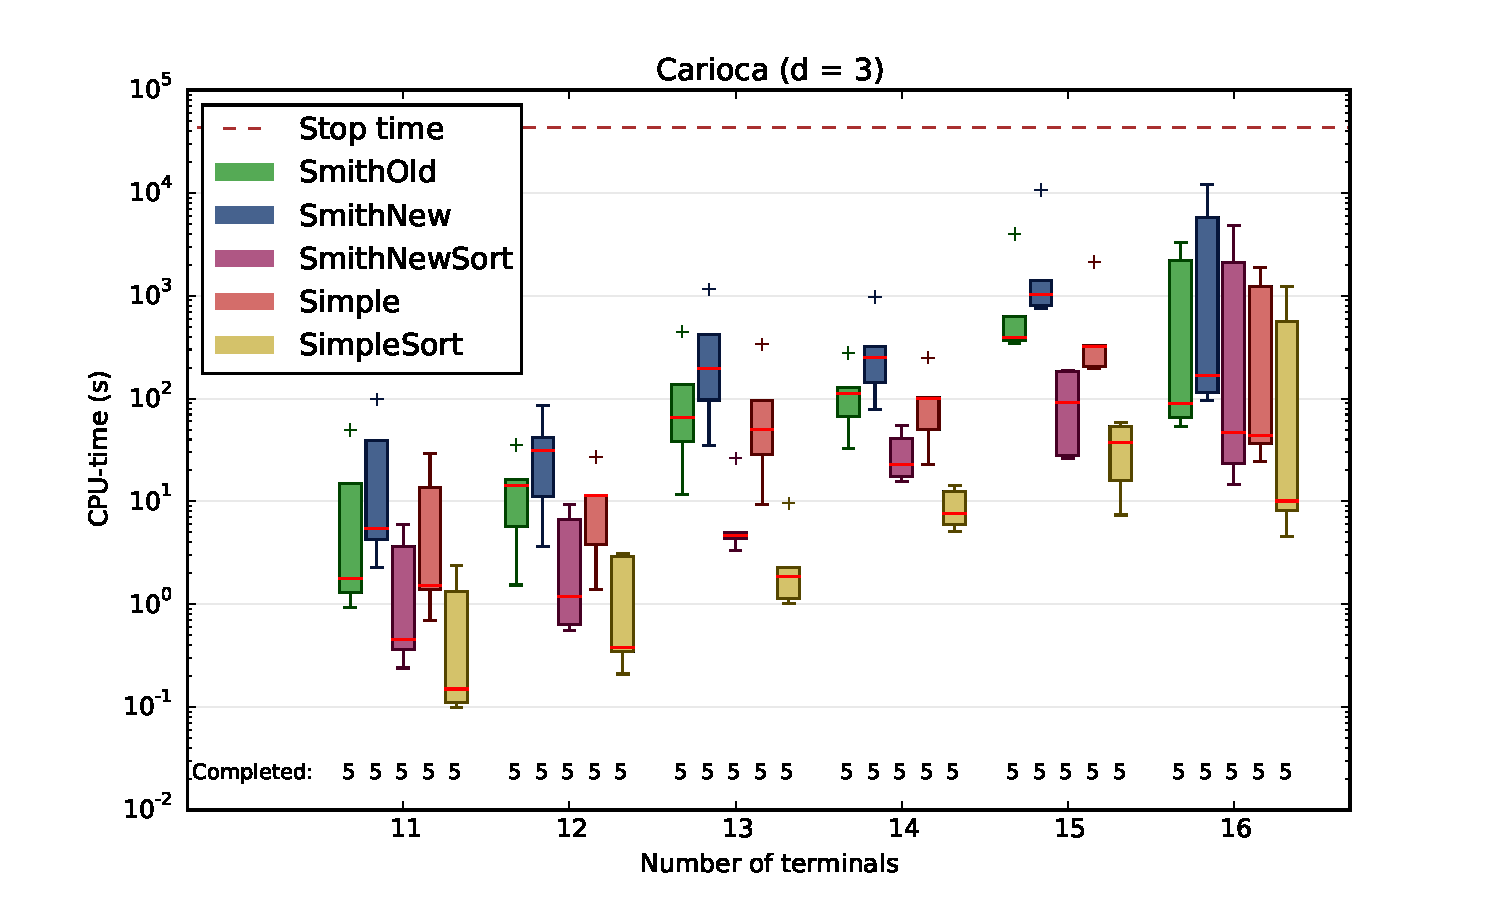
\includegraphics[width=\textwidth]{gfx/boxplots/plot_nvst_boxplot_d3_Carioca_1}
  \caption{Here be dragons.\label{fig:boxplot-d3-carioca-1}}
  \end{subfigure}%
  \begin{subfigure}[t]{0.5\textwidth}
    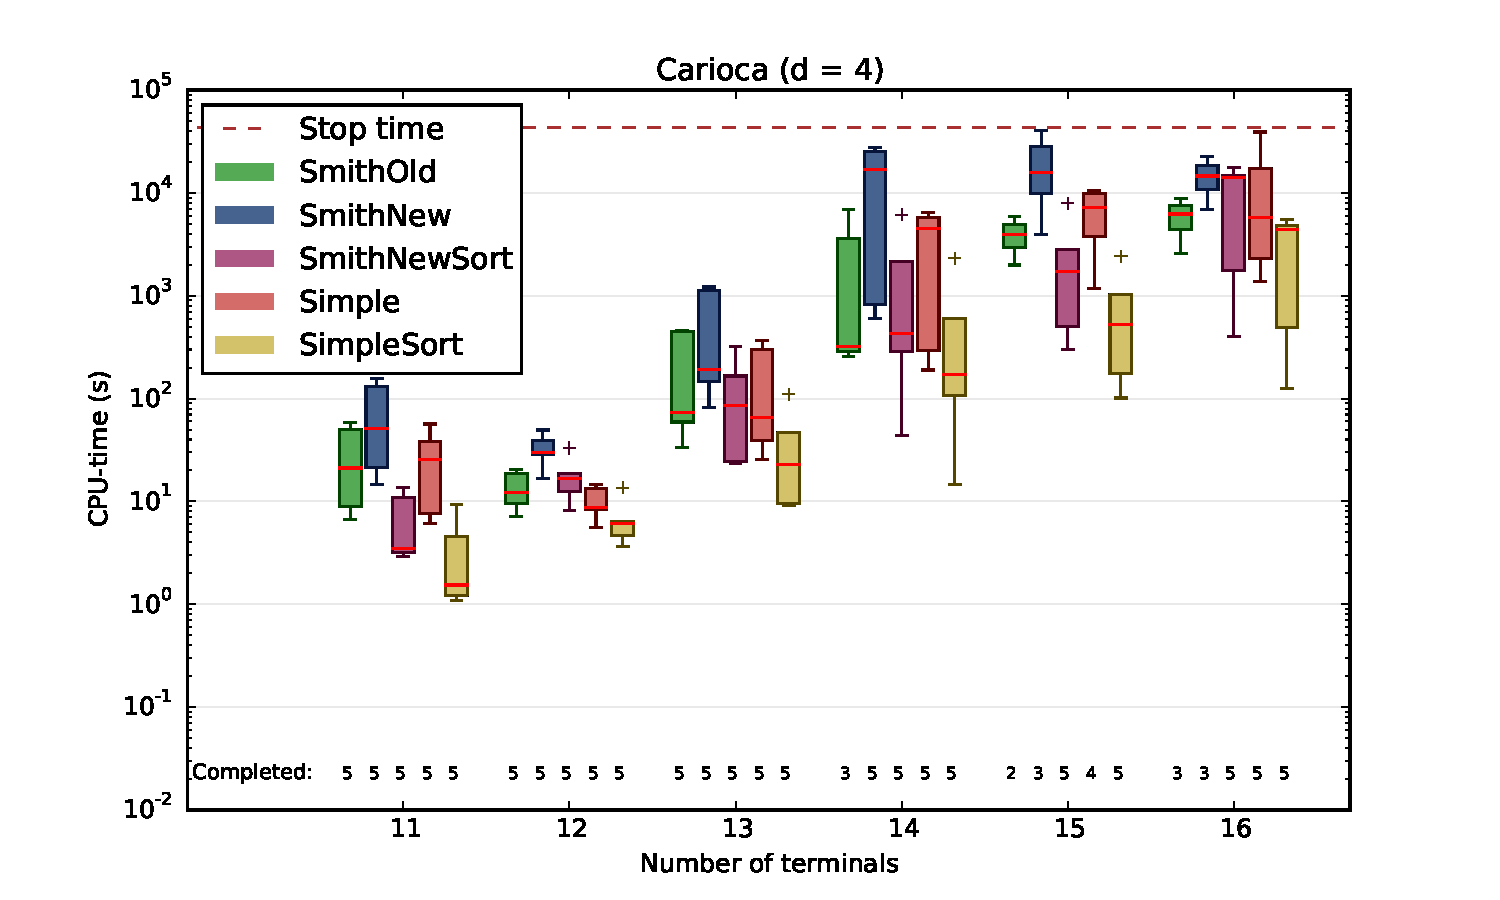
\includegraphics[width=\textwidth]{gfx/boxplots/plot_nvst_boxplot_d4_Carioca_1}
  \caption{Here be dragons.\label{fig:boxplot-d3-carioca-1}}
  \end{subfigure}%
  \caption[Here be dragons]{Here be dragons\label{fig:boxplot-carioca-1}}
\end{figure}

\begin{figure}[htbp]
  \centering
  \begin{subfigure}[t]{0.5\textwidth}
    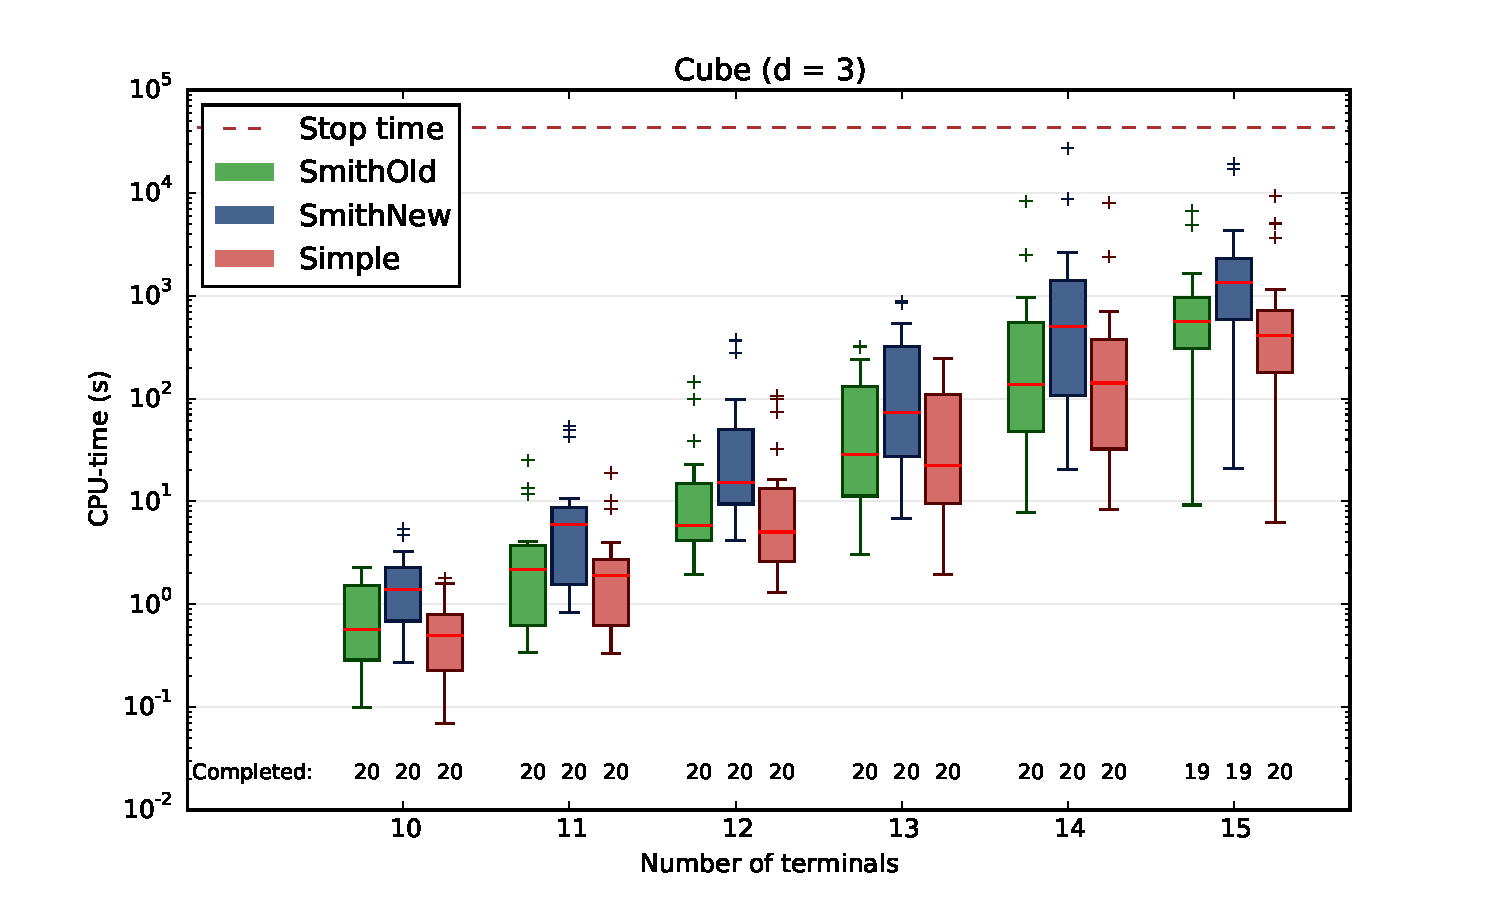
\includegraphics[width=\textwidth]{gfx/boxplots/plot_nvst_boxplot_d3_Cube_1}
  \caption{Here be dragons.\label{fig:boxplot-d3-cube-1}}
  \end{subfigure}%
  \begin{subfigure}[t]{0.5\textwidth}
    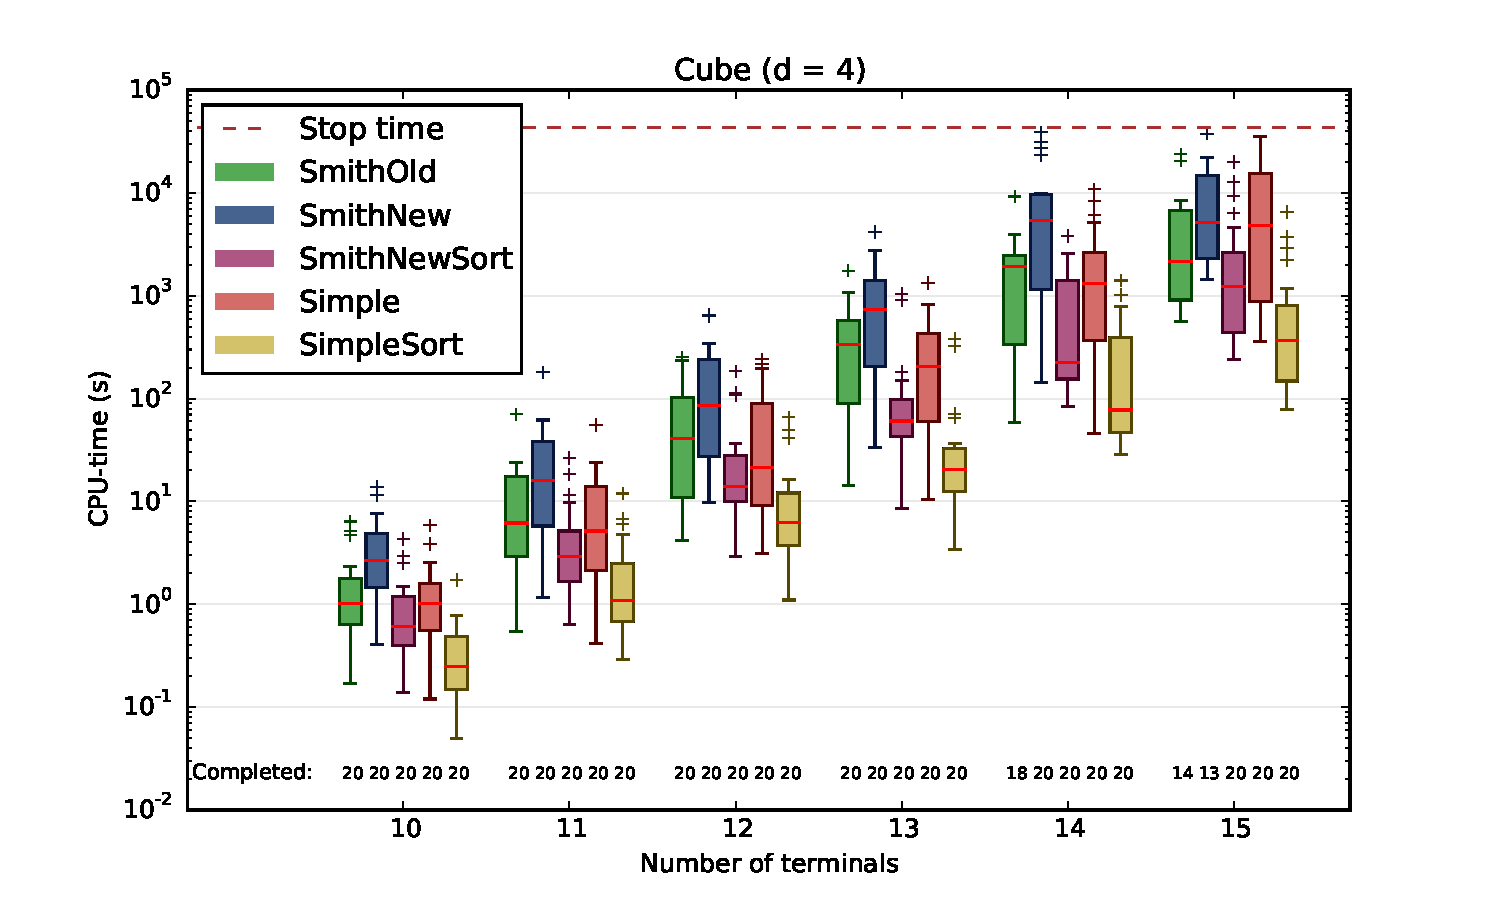
\includegraphics[width=\textwidth]{gfx/boxplots/plot_nvst_boxplot_d4_Cube_1}
  \caption{Here be dragons.\label{fig:boxplot-d3-cube-1}}
  \end{subfigure}%
  \caption[Here be dragons]{Here be dragons\label{fig:boxplot-cube-1}}
\end{figure}

\begin{figure}[htbp]
  \centering
  \begin{subfigure}[t]{0.5\textwidth}
    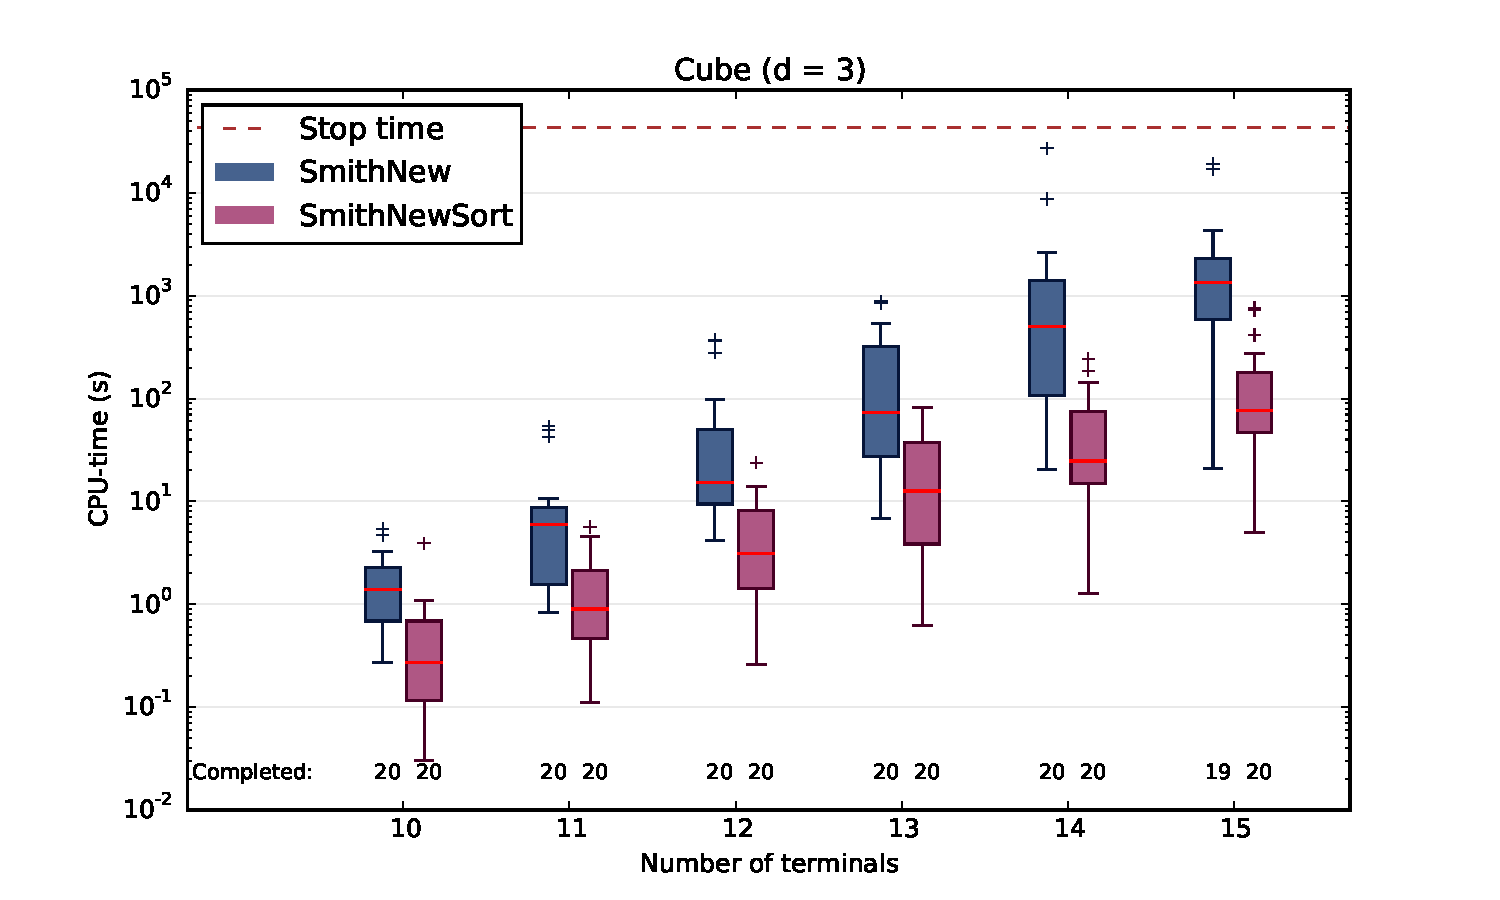
\includegraphics[width=\textwidth]{gfx/boxplots/plot_nvst_boxplot_d3_Cube_2}
  \caption{Here be dragons.\label{fig:boxplot-d3-cube-2}}
  \end{subfigure}%
  \begin{subfigure}[t]{0.5\textwidth}
    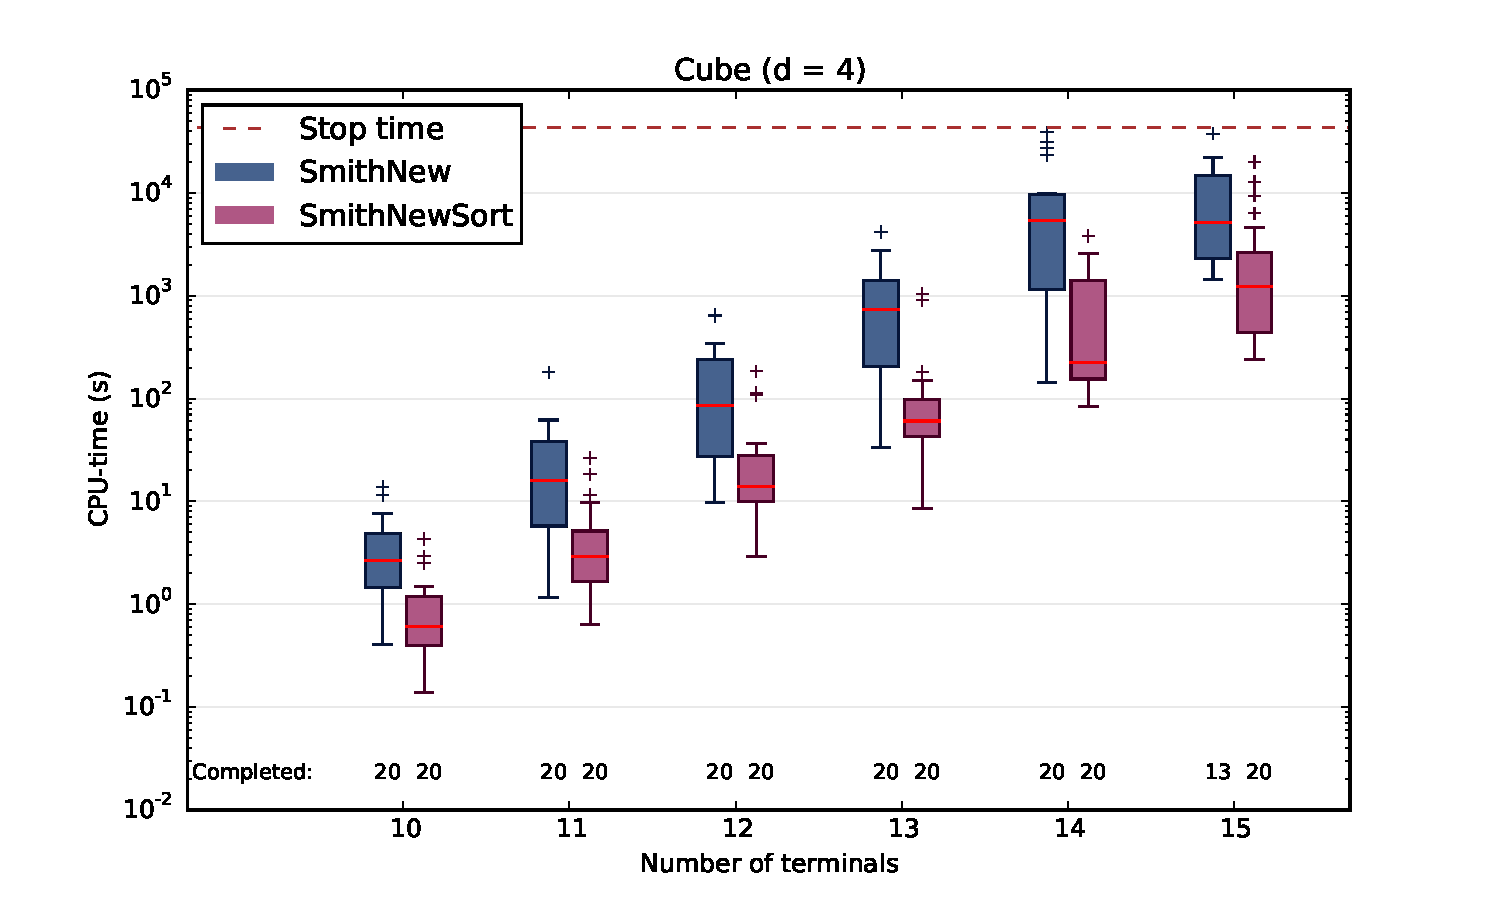
\includegraphics[width=\textwidth]{gfx/boxplots/plot_nvst_boxplot_d4_Cube_2}
  \caption{Here be dragons.\label{fig:boxplot-d3-cube-2}}
  \end{subfigure}%
  \caption[Here be dragons]{Here be dragons\label{fig:boxplot-cube-2}}
\end{figure}

\begin{figure}[htbp]
  \centering
  \begin{subfigure}[t]{0.5\textwidth}
    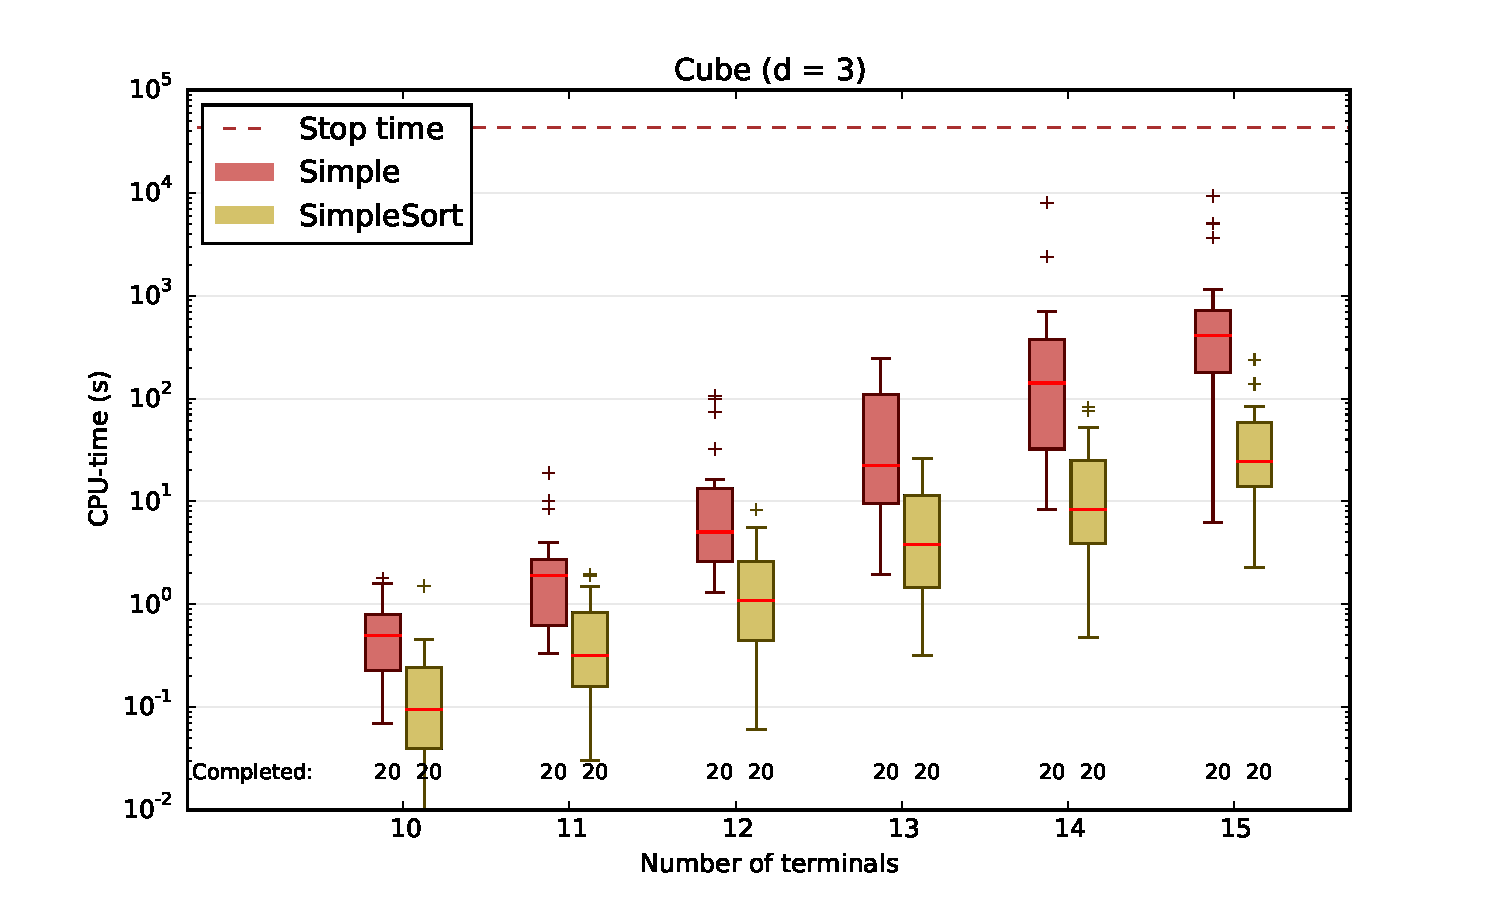
\includegraphics[width=\textwidth]{gfx/boxplots/plot_nvst_boxplot_d3_Cube_3}
  \caption{Here be dragons.\label{fig:boxplot-d3-cube-3}}
  \end{subfigure}%
  \begin{subfigure}[t]{0.5\textwidth}
    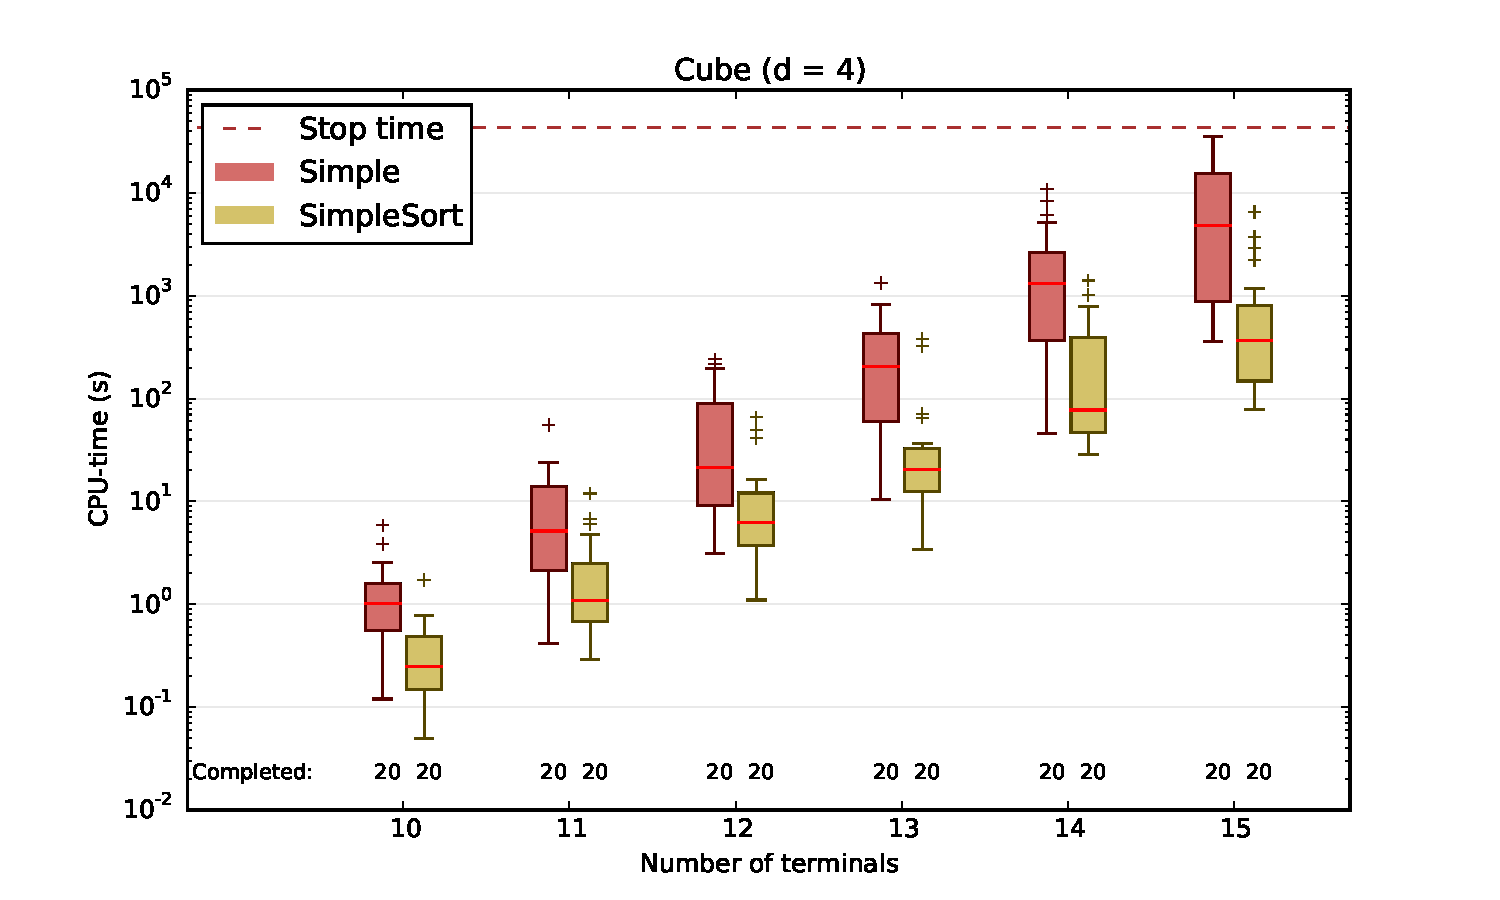
\includegraphics[width=\textwidth]{gfx/boxplots/plot_nvst_boxplot_d4_Cube_3}
  \caption{Here be dragons.\label{fig:boxplot-d3-cube-3}}
  \end{subfigure}%
  \caption[Here be dragons]{Here be dragons\label{fig:boxplot-cube-3}}
\end{figure}

\section{Trees and Iterations}
\label{sec:trees-iterations}

Introduction

\subsection{Trees}
\label{sec:trees}

\begin{table}[htbp]
  \centering
  \begin{tabular}{ccccccc}
    \toprule
         &     & \multicolumn{5}{c}{Method}                               \\
    \cmidrule(l){3-7}
    $n$  & $d$ & Simple & SimpleSort & SmithNew & SmithNewSort & SmithOld \\
    \cmidrule(r){1-2}\cmidrule(l){3-7}
    $10$ & $2$ & $1.04$ & $0.13$     & $1.42$   & $0.17$       & $1.00$   \\
         & $3$ & $1.21$ & $0.25$     & $1.70$   & $0.37$       & $1.00$   \\
         & $4$ & $1.17$ & $0.60$     & $1.61$   & $0.89$       & $1.00$   \\
         & $5$ & $1.54$ & $0.85$     & $2.25$   & $1.34$       & $1.00$   \\
    \cmidrule(r){1-2}
    $11$ & $2$ & $1.05$ & $0.10$     & $1.62$   & $0.13$       & $1.00$   \\
         & $3$ & $1.23$ & $0.19$     & $1.90$   & $0.29$       & $1.00$   \\
         & $4$ & $1.47$ & $0.36$     & $1.97$   & $0.56$       & $1.00$   \\
         & $5$ & $1.54$ & $0.77$     & $2.57$   & $1.22$       & $1.00$   \\
    \cmidrule(r){1-2}
    $12$ & $2$ & $1.17$ & $0.08$     & $1.90$   & $0.11$       & $1.00$   \\
         & $3$ & $1.42$ & $0.16$     & $2.34$   & $0.25$       & $1.00$   \\
         & $4$ & $1.73$ & $0.26$     & $2.83$   & $0.52$       & $1.00$   \\
         & $5$ & $1.53$ & $0.59$     & $2.24$   & $1.11$       & $1.00$   \\
    \cmidrule(r){1-2}
    $13$ & $2$ & $1.11$ & $0.05$     & $2.22$   & $0.09$       & $1.00$   \\
         & $3$ & $1.43$ & $0.12$     & $2.80$   & $0.20$       & $1.00$   \\
         & $4$ & $0.74$ & $0.25$     & $3.19$   & $0.43$       & $1.00$   \\
         & $5$ & $1.66$ & $0.45$     &          & $1.14$       & $1.00$   \\
    \cmidrule(r){1-2}
    $14$ & $2$ & $0.97$ & $0.05$     & $2.63$   & $0.08$       & $1.00$   \\
         & $3$ & $1.61$ & $0.10$     & $3.44$   & $0.19$       & $1.00$   \\
         & $4$ & $1.52$ & $0.16$     &          & $0.39$       & $1.00$   \\
         & $5$ &        &            &          &              &          \\
    \cmidrule(r){1-2}
    $15$ & $2$ & $1.32$ & $0.04$     & $3.12$   & $0.06$       & $1.00$   \\
         & $3$ &        &            &          &              &          \\
         & $4$ &        &            &          &              &          \\
         & $5$ &        &            &          &              &          \\
    \bottomrule
  \end{tabular}
  \caption[Here be dragons]{Here be dragons.\label{tab:trees-sausage}}
\end{table}

\subsection{Iterations}
\label{sec:iterations}

\begin{table}[htbp]
  \centering
  \small
  \begin{tabular}{cccccc}
    \toprule
         & \multicolumn{5}{c}{Method}                               \\
    \cmidrule(l){2-6}
    $n$  & Simple & SimpleSort & SmithNew & SmithNewSort & SmithOld \\
    \cmidrule(r){1-1}\cmidrule(l){2-6}
    $4$  & $0.24$ & $0.25$     & $0.99$   & $0.99$       & $1.00$   \\
    $6$  & $0.34$ & $0.33$     & $0.98$   & $1.01$       & $1.00$   \\
    $8$  & $0.28$ & $0.26$     & $1.38$   & $1.19$       & $1.00$   \\
    $12$ & $0.17$ & $0.12$     & $1.49$   & $1.51$       & $1.00$   \\
    $20$ &        &            &          &              &          \\
    \bottomrule
  \end{tabular}
  \caption[Here be dragons]{Here be dragons.\label{tab:iterations-solids-ratio}}
\end{table}

%%% Local Variables:
%%% mode: latex
%%% TeX-master: "../../main"
%%% End:

{
\abnormalparskip{0pt}
\chapter{Discussion}
\label{cha:discussion}
}

\endChapter{}

%%% Local Variables:
%%% mode: latex
%%% TeX-master: "../../main"
%%% End:

{
\abnormalparskip{0pt}
\chapter{Conclusion}
\label{cha:conclusion}
}

\chapterbreak{}

%%% Local Variables:
%%% mode: latex
%%% TeX-master: "../../main"
%%% End:


\appendix
{ \abnormalparskip{0pt}
\chapter{Proof of Convergence}
\label{cha:proof-convergence} }

Before discussing the convergence we define the length $L$ as is normally the
case, calculated as the sum of all edge lengths. In this case we use the regular
Euclidean ($\mathcal{L}_2$) norm. One could however think to possibly use other
norms, e.g.\ the rectilinear ($\mathcal{L}_1$) norm. Thus

\begin{equation}
  \label{eq:23}
  L(S) = \sum_{j,l : (j,l) \in \mathcal{T}} | p_l - p_j |
\end{equation}

Note that \textcite{smith1992} defines $L$ as a function of the set of
Steiner points $S$ instead of the tree $T$. Here we follow this
convention, as we need the function when we argue about the iteration, in which
only the Steiner points move and the terminals remain fixed. Also remember
that $\mathcal{T} \equiv E(T)$.

\begin{proof}
The proof of convergence is as follows: After the first iteration all Steiner
points lie within the convex hull of the terminals. By the Bolzano-Weierstrass
theorem any infinite sequence of points inside a compact region (such as a
convex hull) has some infinite subsequence approaching a limit point. We
therefore wish to show that the only limit point which can exist, represents
the \ac{rmt} for the underlying topology.

Firstly after each ($i$th) iteration, according to \textcite{smith1992},
$S^{(i+1)}$ exactly minimizes the following quadratic form $Q^{(i)}(S)$
%
\begin{equation}
  Q^{(i)}(S) = \sum_{j,l : (j,l) \in \mathcal{T}, l \in S, j < l }
  \frac{|p_l - p_j|^2}{|p^{(i)}_l - p^{(i)}_j|}
\end{equation}
%
Note that the last two conditions on the sum are redundant and---as far as I can
tell---are only given by \citeauthor{smith1992} to emphasize the way in which
trees are split and edges are numbered. It is easily seen that $Q(S)$ is related to
$L(S)$ in the following way
%
\begin{align}
  Q^{(i)}(S^{(i)})
  &= \sum_{(j,l) \in \mathcal{T}}
    \frac{|p^{(i)}_l - p^{(i)}_j|^2}{|p^{(i)}_l - p^{(i)}_j|} \\
  &= \sum_{(j,l) \in \mathcal{T}} |p^{(i)}_l - p^{(i)}_j| \\
  &= L(S^{(i)}) \label{eq:24}
\end{align}
%
Smith describes that, using \textcite{gilbert1968}'s mechanical model one can
think of $Q$ as the potential energy of a system of ideal springs on the tree
edges, where the force constant of each spring is proportional to the reciprocal
of its original length before each iteration. The $i$th iteration causes all
springs to relax, minimizing $Q^{(i)}$. After several talks with my supervisor,
it is however still a unclear to me that $S^{(i+1)}$ really minimize $Q^{(i)}$.

However as the proof of convergence hinges on this fact\footnote{As we need to
  utilize that $Q^{(i)}(S^{(i)}) \ge Q^{(i)}(S^{(i+1)})$} we can only proceed if
this is the case. Thus I here assume that this is correct. We then do as follows
%
\begin{align}
  L(S^{(i)}) \; &\refequal{eq:24} \; Q^{(i)}(S^{(i)}) \\
                &\ge Q^{(i)}(S^{(i+1)}) \\
                &= \sum_{j, l : (j,l) \in \mathcal{T}}
                  \frac{{\lenpljii}^2}
                  {\lenplji} \\
  \intertext{using that we can add and subtract the same thing without changing
  the equation, we do}
                &= \sum_{j, l : (j,l) \in \mathcal{T}}
                  \frac{{(\lenpljii + \lenplji - \lenplji)}^2}
                  {|p_l^{(i)} - p_j^{(i)}|} \label{eq:25}
\end{align}
%
We then write out and reorder the numerator of the fraction in \cref{eq:25},
here name $\textit{num}$. To further simplify the equation, as it does otherwise
get quite hairy, we define $a = \lenpljii$ and $b = \lenplji$. Thus
%
\begin{align}
  \label{eq:26}
  \textit{num}
  &= {(\lenpljii + \lenplji - \lenplji)}^2 \\
  &= {(a + b - b)}^2 \\
  &= (a^2 + ab - ab) + (ba + b^2 - b^2) + (-ba - b^2 + b^2) \\
  &= (a^2 + b^2 - ab - ab) + (b^2 - b^2 - b^2) + (ab + ba) \\
  &= 2ab - b^2 + {(a - b)}^2
    \intertext{then dividing the numerator again with the denominator from
    \cref{eq:25} $\textit{denom} = \lenplji = b$ we get}
    \frac{\textit{num}}{\textit{denom}}
  &= \frac{2ab - b^2 + {(a - b)}^2}{b} = 2a - b + \frac{{(a-b)}^2}{b} \label{eq:27}
\end{align}
%
Finally we can go back to \cref{eq:25} and insert the fraction we have in
\cref{eq:27}. Thus
%
\begin{align}
  ~(\ref{eq:25})
  &= \sum_{j, l : (j,l) \in \mathcal{T}}
    \left[ 2a - b + \frac{{(a-b)}^2}{b} \right] \\
  &= 2 \sum_{j, l : (j,l) \in \mathcal{T}} \lenpljii -
    \sum_{j, l : (j,l) \in \mathcal{T}} \lenplji \\
  &\quad + \sum_{j, l : (j,l) \in \mathcal{T}}
    \frac{{(\lenpljii - \lenplji)}^2}{\lenplji} \\
  &\refequal{eq:23} \; 2 L(S^{(i+1)}) - L(S^{(i)}) \\
  &\quad + \sum_{j, l : (j,l) \in \mathcal{T}}
    \frac{{(\lenpljii - \lenplji)}^2}{\lenplji} \Leftrightarrow \\
  2 L(S^{(i)}) &\ge 2 L(S^{(i+1)}) \\
  &\quad + \sum_{j, l : (j,l) \in \mathcal{T}}
    \frac{{(\lenpljii - \lenplji)}^2}{\lenplji}
\end{align}
%
As the last sum is obviously non-negative\footnote{The numerator is squared and
  thus non-negative, and the denominator is a length and thus non-negative.}, we
can remove it without the validity of the equation changing, and thus
%
\begin{equation}
  L(S^{(i)}) \ge L(S^{(i+1)})
\end{equation}
%
We now know that performing an iteration, will always either decrease the length
of the tree, or it will remain the same. The only way that it can remain the
same, i.e.\ that we can have equality $L(S^{(i)}) = L(S^{(i+1)})$ is if we are
at a fixed point of the iteration. There are only two types of fixed
points---the optimum\footnote{Which is the \ac{rmt} for this topology.} and
certain places where one or more edges have length zero. As earlier described
the iteration as we have written it is not strictly defined, due to a division
with zero. However according to \citeauthor{smith1992} the singularity is
removable\footnote{How this is the case, is unclear and unexplained by
  \citeauthor{smith1992}. But as I understand it, the singularities are
  removable by his perturbation.}~\cite{removablesingularity} and thus we remove it.

The next part of the proof again hinges on a postulate by \citeauthor{smith1992}
which is not clearly true to me---that the non-optimum fixed points are unstable
in any direction.

Firstly \citeauthor{smith1992} claims that the non-optimum fixed points are
unstable in any $L$-decreasing direction, and thus a small perturbation of the
Steiner points $S$ in any such direction will cause the iteration to
continue. This makes sense as we know that $L$ can never \textit{increase} when
we run the iteration. Thus after decreasing $L$ by a small perturbation, either
we will be past the fixed point and the iteration will continue to decrease, or
we hit another fixed point\footnote{at which point we then again will have to
  use a small perturbation.}. \citeauthor{smith1992} then refers to
\textcite{gilbert1968} who have pointed out that optimizing a pre-specified
Steiner topology is a ``strictly convex'' optimization problem, i.e.\ the only
local optimum is global. This means that there will always be a $L$-decreasing
direction if we are not yet at the optimum.

This currently means we need to find a $L$-decreasing perturbation for
the iteration to continue its convergence. \citeauthor{smith1992} however
further argues that any small step in the opposite direction of a $L$-decreasing
one would also cause the iteration to resume decreasing $L$. The argument for
this is based on the physical spring model of Steiner trees, introduced by
\textcite{gilbert1968}. I have unfortunately not been able to follow the
argument \textcite{smith1992} gives, and after much discussion with my
supervisor Pawel Winter it is still unclear to both of us whether this argument
actually holds.

If we assume that the argument holds, then the iteration, when it is at a
non-optimum fixed point, is unstable in every direction. Thus we have a
$0$-measure\footnote{as we can disregard all these points because of their
  instability.} set of initial iterates which end up at the non-optimal fixed
points. Finally we can the conclude that any Bolzano-Weierstrass subsequence
limit tree must be a fixed point of the iteration. This is done by continuity of
$L$, the iteration function and since the only points where the iteration does
not decrease $L$ are fixed points. However as all non-optimum fixed points are
in the 0-measure set, we have ruled those out and thus the only fixed point is
the optimum.
\end{proof}

%%% Local Variables:
%%% mode: latex
%%% TeX-master: "../../main"
%%% End:

{ \abnormalparskip{0pt}
\chapter{Proof of the Analytical Method for the Fermat-Torricelli Problem}
\label{cha:proof-analyt-meth}
}

\section{2D}
\label{sec:2d-1}

\begin{proof}
To prove \cref{eq:15} the first step is to prove the two following
equations
%
\begin{align}
  \label{eq:16}
  K_1 K_2 + K_1 K_3 + K_2 K_3 &= 2 \sqrt{3} S d\\
  \label{eq:2}
  r_{23}^2 K_1 + r_{13}^2 K_2 + r_{12}^2 K_3 &= 2 S d
\end{align}
%
Both can proven by simply substituting the right hand sides with the definition
of each symbol, i.e.\ through direct computation. Using \cref{eq:16} we can
rewrite \cref{eq:15} as
%
\begin{gather}
  \label{eq:17}
  \left\{
    \begin{array}{c}
  x_\ast = \frac{1}{\frac{1}{K_1} + \frac{1}{K_2} + \frac{1}{K_3}} \left( \frac{x_1}{K_1} +
    \frac{x_2}{K_2} + \frac{x_3}{K_3} \right) \\
  y_\ast = \frac{1}{\frac{1}{K_1} + \frac{1}{K_2} + \frac{1}{K_3}} \left( \frac{y_1}{K_1} +
    \frac{y_2}{K_2} + \frac{y_3}{K_3} \right)
    \end{array}
  \right.  \intertext{Which will be useful in later calculations. The second
    part is to prove that}
  \sqrt{{(x_\ast - x_j)}^2 + {(y_\ast - y_j)}^2} = \frac{K_j}{\sqrt{3 d}},
\quad j \in \{ 1, 2, 3 \}\label{eq:18}
\end{gather}
%
As the calculations are similar for all $j$, only the one for $j = 1$ is shown
here. Thus
%
\begin{align}
  (x_\ast &- x_1)^2
  + {(y_\ast - y_1)}^2 \\
  &\stackrel{\mathclap{(\ref{eq:15})}}{=}
    {\left( \frac{K_1 K_2 K_3}{2 \sqrt{3} S d} \left( \frac{x_1}{K_1} +
    \frac{x_2}{K_2} + \frac{x_3}{K_3} \right) - x_1 \right)}^2 +
    {\left( \frac{K_1 K_2 K_3}{2 \sqrt{3} S d} \left( \frac{y_1}{K_1} +
    \frac{y_2}{K_2} + \frac{y_3}{K_3} \right) - y_1 \right)}^2 \\
  &= {\left( \frac{K_1 K_2 K_3}{2 \sqrt{3} S d} \right)}^2 \left[{\left(
    \frac{x_1}{K_1} + \frac{x_2}{K_2} + \frac{x_3}{K_3} -
    \frac{x_1 2 \sqrt{3} S d}{K_1 K_2 K_3} \right)}^2 + {\left(
    \frac{y_1}{K_1} + \frac{y_2}{K_2} + \frac{y_3}{K_3} -
    \frac{y_1 2 \sqrt{3} S d}{K_1 K_2 K_3} \right)}^2 \right] \\
  &\stackrel{\mathclap{(\ref{eq:16})}}{=}
    {\left( \frac{K_1 K_2 K_3}{2 \sqrt{3} S d} \right)}^2
    \left[ {\left( \frac{x_2}{K_2} + \frac{x_3}{K_3} - \frac{x_1}{K_2} -
    \frac{x_1}{K_3} \right)}^2 + {\left( \frac{y_2}{K_2} + \frac{y_3}{K_3} -
    \frac{y_1}{K_2} - \frac{y_1}{K_3} \right)}^2 \right] \\
  &= {\left( \frac{K_1 K_2 K_3}{2 \sqrt{3} S d} \right)}^2
    \left[ \frac{{(x_2 - x_1)}^2 + {(y_2 - y_1)}^2}{K_2^2} +
    \frac{{(x_3 - x_1)}^2 + {(y_3 - y_1)}^2}{K_3^2} \right. \\
  &\hspace{7em} \left. + \; 2 \frac{(x_2 - x_1)(x_3 - x_1) +
    (y_2 - y_1)(y_3 - y_1)}{K_2 K_3} \right] \\
  &\stackrel{\mathclap{(\ref{eq:1})}}{=}
    {\left( \frac{K_1 K_2 K_3}{2 \sqrt{3} S d} \right)}^2
    \left[ \frac{r_{12}^2}{K_2^2} + \frac{r_{13}^2}{K_3^2} +
    \frac{r_{12}^2 + r_{13}^2 - r_{23}^2}{K_2 K_3} \right] \label{eq:30} \\
  &= \frac{K_1^2}{{(2 \sqrt{3} S d)}^2}
    \left[ r_{12}^2 K_3^2 + r_{13}^2 K_2^2 +
    (r_{12}^2 + r_{13}^2 - r_{23}^2) K_2 K_3 \right] \\
  &= \frac{K_1^2}{{(2 \sqrt{3} S d)}^2}
    \left[ (r_{12}^2 K_3 + r_{13}^2 K_2) (K_2 + K_3) -
    r_{23}^2 K_2 K_3 \right] \\
  &\stackrel{\mathclap{(\ref{eq:2})}}{=}
    \frac{K_1^2}{{(2 \sqrt{3} S d)}^2}
    \left[ (2 S d - r_{23}^2 K_1) (K_2 + K_3) - r_{23}^2 K_2 K_3 \right] \\
  &= \frac{K_1^2}{{(2 \sqrt{3} S d)}^2}
    \left[ 2 S d (K_2 + K_3) - r_{23}^2 (K_1 K_2 + K_1 K_3 + K_2 K_3) \right] \\
  &\stackrel{\mathclap{(\ref{eq:16})}}{=}
    \frac{K_1^2}{{(2 \sqrt{3} S d)}^2}
    \left[ 2 S d (K_2 + K_3) - 2 \sqrt{3} r_{23}^2 S d \right] \\
  &= \frac{2 S d K_1^2}{{(2 \sqrt{3} S d)}^2}
    \left[ K_2 + K_3 - \sqrt{3} r_{23}^2 \right] \\
  &\stackrel{\mathclap{(\ref{eq:3})}}{=}
    \frac{K_1^2}{6 S d}
    \left[ 2 S \right] \\
  &= \frac{K_1^2}{3 d}
\end{align}
%
Thus
%
\begin{equation}
  \label{eq:29}
  \sqrt{{(x_\ast - x_1)}^2 + {(y_\ast - y_1)}^2}
  = \sqrt{\frac{K_1^2}{3 d}} = \frac{K_1}{\sqrt{3 d}}
\end{equation}
%
To finish the proof one would also have to show that $K_1, K_2, K_3$ are
nonnegative. The proof of this can be found in~\cite[p.~5-6]{uteshev2014}.

We can now prove \cref{eq:15}, by substituting it into \cref{eq:13}. As the
equations are similar for $x$ and $y$, only $x$ is shown here
%
\begin{align}
  0
  &= \frac{(x_\ast - x_1)}{\sqrt{{(x_\ast - x_1)}^2 + {(y_\ast - y_1)}^2}} +
    \frac{(x_\ast - x_2)}{\sqrt{{(x_\ast - x_2)}^2 + {(y_\ast - y_2)}^2}} +
    \frac{(x_\ast - x_3)}{\sqrt{{(x_\ast - x_3)}^2 + {(y_\ast - y_3)}^2}} \\
  &\stackrel{\mathclap{(\ref{eq:18})}}=
    \frac{(x_\ast - x_1)}{\frac{K_1}{\sqrt{3 d}}} +
    \frac{(x_\ast - x_2)}{\frac{K_2}{\sqrt{3 d}}} +
    \frac{(x_\ast - x_3)}{\frac{K_3}{\sqrt{3 d}}} \\
  &= \sqrt{3 d} \left[
    \frac{x_\ast - x_1}{K_1} +
    \frac{x_\ast - x_2}{K_2} +
    \frac{x_\ast - x_3}{K_3} \right] \\
  &= \sqrt{3 d} \left[
    x_\ast \left( \frac{1}{K_1} + \frac{1}{K_2} + \frac{1}{K_3} \right) -
    \left( \frac{x_1}{K_1} + \frac{x_2}{K_2} + \frac{x_3}{K_3} \right)
    \right] \\
  &\stackrel{\mathclap{(\ref{eq:17})}}=
    \sqrt{3 d} \left[
    \frac{1}{\frac{1}{K_1} + \frac{1}{K_2} + \frac{1}{K_3}} \left( \frac{x_1}{K_1} +
    \frac{x_2}{K_2} + \frac{x_3}{K_3} \right)
    \left( \frac{1}{K_1} + \frac{1}{K_2} + \frac{1}{K_3} \right) -
    \left( \frac{x_1}{K_1} + \frac{x_2}{K_2} + \frac{x_3}{K_3} \right)
    \right] \\
  &= \sqrt{3 d} \left[
    \frac{1}{\frac{1}{K_1} + \frac{1}{K_2} + \frac{1}{K_3}}
    \left( \frac{1}{K_1} + \frac{1}{K_2} + \frac{1}{K_3} \right) -
    1 \right] \\
  &= \sqrt{3 d} \left[ 1 - 1 \right] = 0
\end{align}
%
As can be seen \cref{eq:15} is a solution to \cref{eq:13}, and thus it minimizes
$F(x,y)$.
\end{proof}

\section{$d$-Space}
\label{sec:d-space}

\begin{proof}
As before to prove \cref{eq:5} (and thus \cref{eq:8}) the first step once
again is to prove \cref{eq:16} and \cref{eq:2}. These can as before be
established through direct computation, i.e.\ by simply substituting the
expressions for their definitions, until both sides only contain distances,
after which the two sides can be seen to be equal. Using \cref{eq:16} we can
rewrite \cref{eq:5} as
%
\begin{gather}
    x_{(\ast, j)} = \frac{1}{\frac{1}{K_1} + \frac{1}{K_2} + \frac{1}{K_3}} \left( \frac{x_{(1,j)}}{K_1} +
  \frac{x_{(2,j)}}{K_2} + \frac{x_{(3,j)}}{K_3} \right), \quad 0 < j \le
d\label{eq:10}
\intertext{similarly to \cref{eq:17} in the 2D version. Secondly we wish
  to prove that}
  \sqrt{\sum_{i = 1}^d {(x_{(\ast,i)} - x_{j,i})}^2} = \frac{K_j}{\sqrt{3 d}
  }, \quad j \in \{ 1, 2, 3 \}\label{eq:19}
\end{gather}
As the calculations are similar for all $j$, only the one for $j = 1$ is shown
here. Thus
%
\begin{align}
  \sum_{i=1}^d (x_{(\ast,i)} &- x_{(1,i)})^2 \\
  &= \sum_{i=1}^d { \left( \frac{K_1 K_2 K_3}{2 \sqrt{3} S d}
    \left( \frac{x_{(1,i)}}{K_1} + \frac{x_{(2,i)}}{K_2} + \frac{x_{(3,i)}}{K_3}
    \right) - x_{(1,i)} \right) }^2 \\
  &= { \left( \frac{K_1 K_2 K_3}{2 \sqrt{3} S d} \right) }^2 \left[ \sum_{i=1}^d
    { \left( \frac{x_{(1,i)}}{K_1} + \frac{x_{(2,i)}}{K_2} +
    \frac{x_{(3,i)}}{K_3} - \frac{x_{(1,i)} 2 \sqrt{3} S d}{K_1 K_2 K_3}
    \right) }^2 \right] \\
  &\stackrel{\mathclap{(\ref{eq:16})}}{=}
    {\left( \frac{K_1 K_2 K_3}{2 \sqrt{3} S d} \right)}^2 \left[ \sum_{i=1}^d
    {\left( \frac{x_{(2,i)}}{K_2} + \frac{x_{(3,i)}}{K_3} - \frac{x_{(1,i)}}{K_2} -
    \frac{x_{(1,i)}}{K_3} \right)}^2 \right] \\
  &= {\left( \frac{K_1 K_2 K_3}{2 \sqrt{3} S d} \right)}^2 \left[ \sum_{i=1}^d
    \left( \frac{{(x_{(2,i)} - x_{(1,i)})}^2}{K_2^2} +
    \frac{{(x_{(3,i)} - x_{(1,i)})}^2}{K_3^2} \right. \right. \\
  &\hspace{7em} \left. \left. + \; 2 \frac{(x_{(2,i)} - x_{(1,i)})(x_{(3,i)} -
    x_{(1,i)})}{K_2 K_3} \right) \right] \\
  &= {\left( \frac{K_1 K_2 K_3}{2 \sqrt{3} S d} \right)}^2
    \left[ \frac{\sum_{i=1}^d {(x_{(2,i)} - x_{(1,i)})}^2}{K_2^2} +
    \frac{\sum_{i=1}^d {(x_{(3,i)} - x_{(1,i)})}^2}{K_3^2} \right. \\
  &+ \left. \frac{ \sum_{i=1}^d {(x_{(2,i)} - x_{(1,i)})}^2 +
    \sum_{i=1}^d {(x_{(3,i)} - x_{(1,i)})}^2 -
    \sum_{i=0}^d {(x_{(2,i)} - x_{(3,i)})}^2}{K_2 K_3} \right] \\
  &\stackrel{\mathclap{(\ref{eq:14})}}{=}
    {\left( \frac{K_1 K_2 K_3}{2 \sqrt{3} S d} \right)}^2
    \left[ \frac{r_{12}^2}{K_2^2} + \frac{r_{13}^2}{K_3^2} +
    \frac{r_{12}^2 + r_{13}^2 - r_{23}^2}{K_2 K_3} \right] \\
  \intertext{As this point we have exactly the same as in \cref{eq:30} and thus
  we can conclude}
  &= \frac{K_1^2}{3 d}
\end{align}
%
From here we can show that \cref{eq:5} is a solution to \cref{eq:7} in the
exactly the same way as
we proved that \cref{eq:15} was a solution to \cref{eq:13}, by substituting
\cref{eq:5} into \cref{eq:7} and using \cref{eq:10} and \cref{eq:19}.
\end{proof}

%%% Local Variables:
%%% mode: latex
%%% TeX-master: "../../main"
%%% End:

\chapter{Source Code}
\label{cha:source-code}

\newmintedfile[golang]{go}{
  frame=lines,
  framesep=2mm,
  fontsize=\footnotesize,
  linenos,
  tabsize=4,
  baselinestretch=0.8,
}

\golang[label=point.go]{sourcecode/smt/point.go}
\golang[label=edge.go]{sourcecode/smt/edge.go}
\golang[label=helpers.go]{sourcecode/smt/helpers.go}
\golang[label=tree.go]{sourcecode/smt/tree.go}
\golang[label=optimize.go]{sourcecode/smt/optimize.go}
\golang[label=main.go]{sourcecode/main.go}

%%% Local Variables:
%%% mode: latex
%%% TeX-master: "../../main"
%%% End:


%------------------------------------------------------------------------------
%	POST-CONTENT  - APPENDIX AND BIBLIOGRAPHY
%------------------------------------------------------------------------------

\backmatter%

\printbibliography%

\end{document}

%%% Local Variables:
%%% mode: latex
%%% TeX-master: t
%%% End:
